\section{Partielle Ableitung}
\subsection*{Ableitung: Rückblick und Erweiterung}

Wir erinnern zunächst an den Begriff der Ableitung bei einer Funktion in einer Variablen: Definitionsgemäss wird der Grenzwert
\[
	f'(x_0) = \lim_{h \to 0} \frac{f(x_0 + h) - f(x_0)}{h}
\]
als \textbf{erste Ableitung} der Funktion \( f \) an der Stelle \( x_0 \) bezeichnet.

Aus geometrischer Sicht lässt sich diese Ableitung als \textbf{Steigung der Kurventangente} im Punkt \( P(x_0, y_0) \) deuten.

\medskip

Betrachtet man nun eine Funktion \( f \colon \mathbb{R}^2 \to \mathbb{R} \), dann merkt man schnell, dass man die Idee der Ableitung als Steigung der Tangente nicht ohne Weiteres übernehmen kann. Im Gegensatz zum eindimensionalen Fall gibt es nun nämlich \textbf{unendlich viele Tangenten}, die durch einen gegebenen Punkt \( P = (x_0, y_0, f(x_0, y_0)) \) verlaufen.

% Betrachtet man nun eine Funktion \( f \colon \mathbb{R}^2 \to \mathbb{R} \), dann merkt man schnell, dass man die Definition für die Ableitung nicht ohne Weiteres übernehmen kann. Sowohl die formale Definition als auch die geometrische Interpretation lassen sich nicht direkt übertragen:

% \begin{itemize}
%   \item Die Inputs sind Vektoren. Der Ausdruck
%   \[
%   \lim_{\vec{h} \to 0} \frac{f((x_0, y_0) + \vec{h}) - f(x_0, y_0)}{\vec{h}}
%   \]
%   ist \textbf{nicht definiert}, da eine Division durch einen Vektor nicht sinnvoll ist.

%   \item Im Gegensatz zum eindimensionalen Fall gibt es nun \textbf{unendlich viele Tangenten}, die durch einen gegebenen Punkt \( P = (x_0, y_0, f(x_0, y_0)) \) verlaufen.
% \end{itemize}

Die Abbildung zeigt in \textcolor{red}{Rot} und in \textcolor{blue}{Blau} die Tangenten in die Koordinatenrichtungen sowie in \textcolor{black}{Schwarz} die Tangente in Richtung der ersten Winkelhalbierenden dieser Koordinatenrichtungen.
\begin{center}
	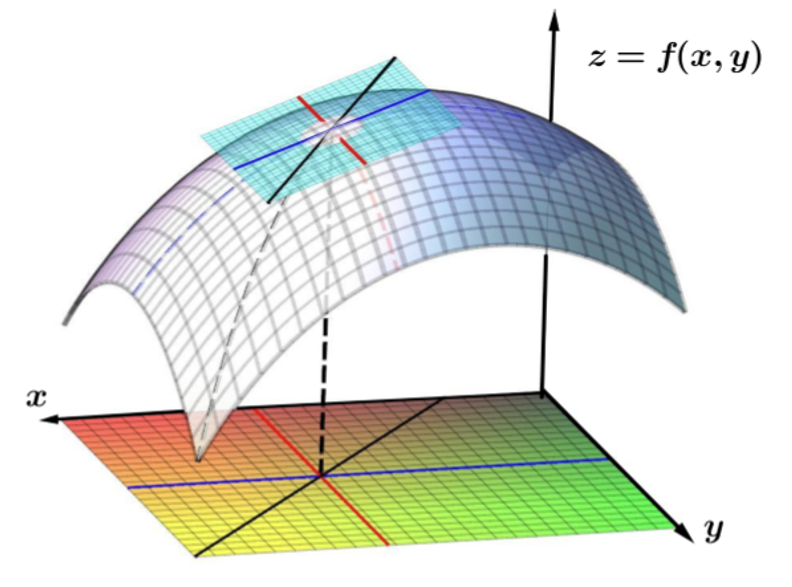
\includegraphics[width = 0.5 \textwidth]{media/GraphTangentialebene.png}
\end{center}

Die Steigung wird im Allgemeinen in verschiedenen Richtungen unterschiedlich sein. Man erhält also für jede Richtung eine eigene Ableitung!

















\subsection{Partielle Ableitungen in Koordinatenrichtungen}

Wir betrachten zuerst die Ableitungen in Richtung der Koordinatenachsen.


Der Graph der Funktion
\[
	f(x, y) = 1 - 3x^2 - y^2 + 5 \cdot \sin(xy)
\]
ist unten dargestellt.

Stellen Sie sich den Graphen der Funktion \( f \) als ein Gelände über der \( (x, y) \)-Ebene vor. Ein Wanderer befindet sich im Punkt
\[
	P = (1, 1, f(1, 1))
\]
und läuft in der gezeichneten Richtung, also \textbf{parallel zur \( xz \)-Ebene} (d.\,h. \( y = \text{konstant} \)).

\begin{center}
	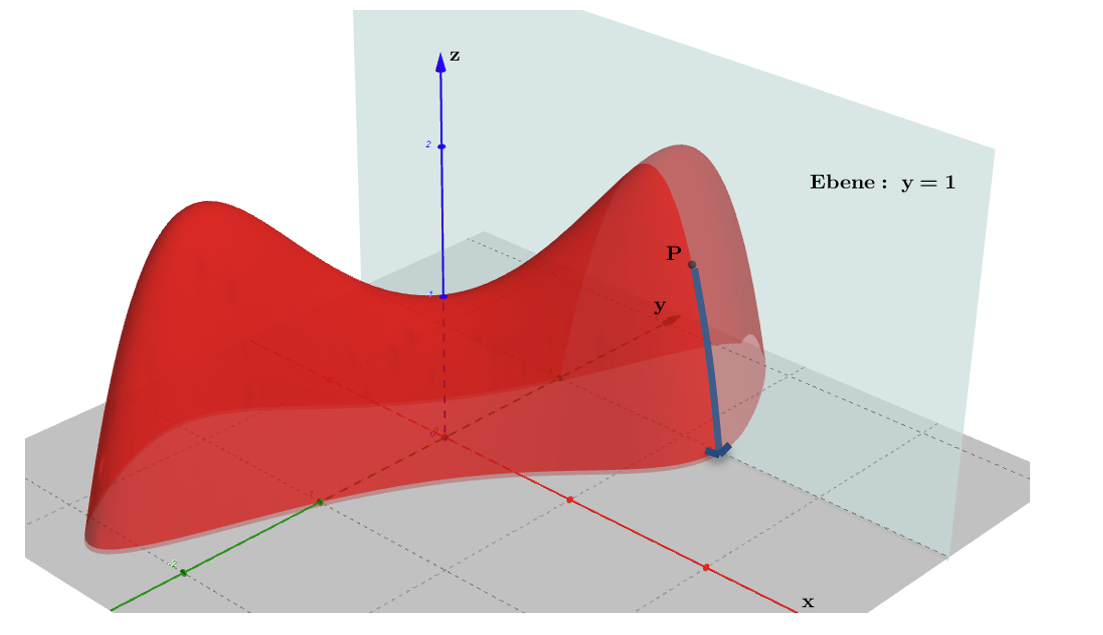
\includegraphics[width = 0.5\textwidth]{media/IntroPartielleAbleitung.png}
\end{center}

Wie steil ist sein Weg?

\medskip

Der Weg, dem der Wanderer folgt, entspricht dem Graphen der \textbf{partiellen Abbildung}
\[
	F_1(x) = f(x, 1)
	= 1 - 3x^2 - 1 + 5 \cdot \sin(x)
	= 5 \cdot \sin(x) - 3x^2
\]

\begin{center}
	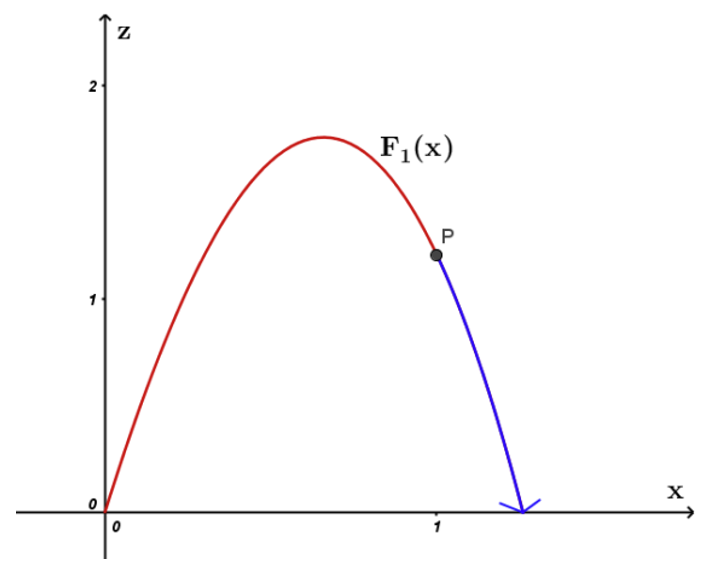
\includegraphics[width = 0.5\textwidth]{media/IntroPartielleAbleitung-Schnittkurve.png}
\end{center}



Die gesuchte Steigung ist nun die Steigung der Tangente an den Graphen von \( F_1 \) an der Stelle \( x = 1 \). Diese ist gleich der Ableitung:

\[
	F_1'(x) = 5 \cdot \cos(x) - 6x
	\quad \Rightarrow \quad
	F_1'(1) = 5 \cdot \cos(1) - 6 \approx -3.3
\]



Ein anderer Wanderer befindet sich im Punkt \( P = (x_0, y_0, f(x_0, y_0)) \) und läuft in dieselbe Richtung, also \textbf{in positive \( x \)-Richtung}. Wie steil ist sein Weg?

Die partielle Abbildung für festes \( y = y_0 \) lautet:
\[
	F_{y_0}(x) = f(x, y_0)
	= 1 - 3x^2 - y_0^2 + 5 \cdot \sin(x y_0)
\]

Die Steigung ergibt sich durch die Ableitung:
\[
	F_{y_0}'(x) = 5 \cdot \cos(x y_0) \cdot y_0 - 6x
	\quad \Rightarrow \quad
	F_{y_0}'(x_0) = 5 \cdot \cos(x_0 y_0) \cdot y_0 - 6x_0
\]

Diese Grösse nennt man die \textbf{partielle Ableitung} von \( f \) nach \( x \) an der Stelle \( (x_0, y_0) \).

\begin{definition}
	{Partielle Ableitung}{}
	Sei \( f \colon \mathbb{R}^2 \to \mathbb{R} \) eine Funktion und sei \( (x_0, y_0) \) eine Stelle im Definitionsbereich von \( f \).

	Falls die partiellen Abbildungen
	\[
		F_{y_0}(x) = f(x, y_0) \quad \text{bzw.} \quad F_{x_0}(y) = f(x_0, y)
	\]
	differenzierbar sind, so nennt man ihre Ableitungen die \textbf{partiellen Ableitungen} von \( f \) an der Stelle \( (x_0, y_0) \).

	Man bezeichnet sie durch die Symbole
	\[
		%f_x(x_0, y_0) \quad \text{oder} \quad 
		\frac{\partial f}{\partial x}(x_0, y_0) \qquad \text{bzw.} \qquad
		%f_y(x_0, y_0) \quad \text{oder} \quad 
		\frac{\partial f}{\partial y}(x_0, y_0)
	\]

	Formal sind sie als Grenzwerte definiert:
	\[
		\frac{\partial f}{\partial x}(x_0, y_0) = \lim_{\Delta x \to 0} \frac{f(x_0 + \Delta x, y_0) - f(x_0, y_0)}{\Delta x}
	\]
	\[
		\frac{\partial f}{\partial y}(x_0, y_0)= \lim_{\Delta y \to 0} \frac{f(x_0, y_0 + \Delta y) - f(x_0, y_0)}{\Delta y}
	\]

\end{definition}
Um die partielle Ableitung von \( f \) nach einer Variablen, z.\,B. nach \( x \), zu berechnen,
denkt man sich alle anderen Variablen als konstant und leitet dann mit den üblichen Differentiationsregeln nach \( x \) ab.


\begin{bsp}
	{}{}
	Gegeben sei die Funktion
	\[
		f(x, y) = e^{x^2 + 2y}
	\]

	\vspace*{3cm}

	% Für die partielle Ableitung nach \( x \) betrachtet man \( y \) als konstant und leitet mit der Kettenregel ab:
	% \[
	% \frac{\partial f}{\partial x}(x, y) = e^{x^2 + 2y} \cdot 2x
	% \]

	% Analog ergibt sich die partielle Ableitung nach \( y \):
	% \[
	% \frac{\partial f}{\partial y}(x, y) = e^{x^2 + 2y} \cdot 2
	% \]
\end{bsp}

\begin{bsp}
	{}{}
	Gegeben sei die Funktion
	\[
		f(x, y) = \sin\left(\frac{x}{y}\right)
	\]

	\vspace*{5cm}


	% Dann gilt:
	% \[
	% \frac{\partial f}{\partial x}(x, y) = \cos\left(\frac{x}{y}\right) \cdot \frac{1}{y}
	% \]

	% \[
	% \frac{\partial f}{\partial y}(x, y) = \cos\left(\frac{x}{y}\right) \cdot \left(-\frac{x}{y^2}\right)
	% \]
\end{bsp}

\begin{ueb}
	{}{}

	\begin{enumerate}
		\item Bestimmen Sie die partiellen Ableitungen der folgenden Funktionen:
		      \begin{enumerate}
			      \item \( f(x, y) = (x^2 - 1)(y + 2) \)
			      \item \( f(x, y) = (xy - 1)^2 \)
			      \item \( f(t, \alpha) = \cos(2\pi t - \alpha) \)
			      \item \( h(r, s) = \dfrac{2rs + r^2}{s + r} \)
			      \item \( g(a, b) = \ln(a) \cdot (2a - b) \)
		      \end{enumerate}

		\item Untersuchen Sie den Graphen von \( f(x, y) = (x^2 - 1)(y + 2) \) (siehe Aufgabe 1a) mit GeoGebra.
		      \begin{enumerate}
			      \item Es gilt: \( \frac{\partial f}{\partial x}(0, y) = 0 \). Woran erkennt man das im Graphen?
			      \item Es gilt: \( \frac{\partial f}{\partial x}(1, -2) = \frac{\partial f}{\partial y}(1, -2) = 0 \). Woran erkennt man das im Graphen?
		      \end{enumerate}

		\item Bestimmen Sie alle Funktionen \( f \), für die jeweils gilt:
		      \begin{enumerate}
			      \item \( \frac{\partial f}{\partial x}(x, y) = 0 \)
			      \item \( \frac{\partial f}{\partial x}(x, y) = \frac{\partial f}{\partial y}(x, y) = 0 \)
			      \item \( \frac{\partial f}{\partial y}(x, y) = x^2 \sin(xy) \)
		      \end{enumerate}
	\end{enumerate}
\end{ueb}
\clearpage
\emph{Lösungen:}


\begin{enumerate}
	\item Partielle Ableitungen:
	      \begin{enumerate}
		      \item Für \( f(x, y) = (x^2 - 1)(y + 2) \):
		            \[
			            \frac{\partial f}{\partial x}(x, y) = 2x(y + 2), \quad
			            \frac{\partial f}{\partial y}(x, y) = x^2 - 1
		            \]

		      \item Für \( f(x, y) = (xy - 1)^2 \):
		            \[
			            \frac{\partial f}{\partial x}(x, y) = 2(xy - 1)y, \quad
			            \frac{\partial f}{\partial y}(x, y) = 2(xy - 1)x
		            \]

		      \item Für \( f(t, \alpha) = \cos(2\pi t - \alpha) \):
		            \[
			            \frac{\partial f}{\partial t}(t, \alpha) = -\sin(2\pi t - \alpha) \cdot 2\pi, \quad
			            \frac{\partial f}{\partial \alpha}(t, \alpha) = \sin(2\pi t - \alpha)
		            \]

		      \item Für \( h(r, s) = \dfrac{2rs + r^2}{s + r} \):
		            \[
			            \frac{\partial h}{\partial r}(r, s) = \frac{2s^2 + r^2 + 2rs}{(s + r)^2}, \quad
			            \frac{\partial h}{\partial s}(r, s) = \frac{r^2}{(s + r)^2}
		            \]

		      \item Für \( g(a, b) = \ln(a) \cdot (2a - b) \):
		            \[
			            \frac{\partial g}{\partial a}(a, b) = 2\ln(a) + \frac{2a - b}{a}, \quad
			            \frac{\partial g}{\partial b}(a, b) = -\ln(a)
		            \]
	      \end{enumerate}
	\item \dots

	\item Allgemeine Lösungen:
	      \begin{enumerate}
		      \item Alle Funktionen, die unabhängig von \( x \) sind, also:
		            \[
			            f(x, y) = g(y)
		            \]

		      \item Alle konstanten Funktionen:
		            \[
			            f(x, y) = C, \quad \text{für ein } C \in \mathbb{R}
		            \]

		      \item Eine Funktion mit \( \frac{\partial f}{\partial y}(x, y) = x^2 \sin(xy) \) ist:
		            \[
			            f(x, y) = -x \cos(xy) + C
		            \]
	      \end{enumerate}
\end{enumerate}


























\subsection{Linearisierung und Tangentialebene}

Unter \emph{Linearisieren} versteht man die Approximation komplexer Funktionen durch eine lineare Funktion.

Das Linearisieren bei Funktionen zweier Variablen erfolgt vollkommen analog zum Linearisieren bei Funktionen einer Variablen.

Ist \( f \) eine Funktion einer Variablen, so approximiert man sie in der Nähe der Stelle \( x_0 \) durch die Tangente \( t(x) \), wobei die Gleichung der Tangente dem Taylorpolynom 1. Grades entspricht:
\[
	t(x) = f(x_0) + f'(x_0) \cdot (x - x_0)
\]

Ist \( f \) eine Funktion zweier Variablen, so linearisiert man diese an der Stelle \( (x_0, y_0) \), indem man sie durch diejenige lineare Funktion ersetzt, deren Graph gerade die Tangentialebene an den Graphen von \( f \) im Punkt
\[
	P = (x_0, y_0, f(x_0, y_0))
\]
ist.

Die Tangentialebene über der Stelle \( (x_0, y_0) \) besteht aus den Tangenten derjenigen Funktionen, die man durch Einschränkung von \( f \) entlang aller möglichen Geraden durch \( (x_0, y_0) \) erhält.

Die lineare Ersatzfunktion (deren Graph die Tangentialebene ist) besitzt folgende Eigenschaften:
\begin{itemize}
	\item ihr Wert in \( (x_0, y_0) \) ist \( f(x_0, y_0) \),
	\item ihre partielle Ableitung nach \( x \) ist \( \frac{\partial f}{\partial x} (x_0, y_0) \),
	\item ihre partielle Ableitung nach \( y \) ist \( \frac{\partial f}{\partial y} (x_0, y_0) \).
\end{itemize}

Diese drei Eigenschaften bestimmen die lineare Ersatzfunktion von \( f \) in \( (x_0, y_0) \) eindeutig. Sie ist gegeben durch:
\[
	T_{(x_0, y_0)}(x, y) = f(x_0, y_0) + \frac{\partial f}{\partial x} (x_0, y_0) \cdot (x - x_0) + \frac{\partial f}{\partial y} (x_0, y_0) \cdot (y - y_0)
\]

\begin{center}
	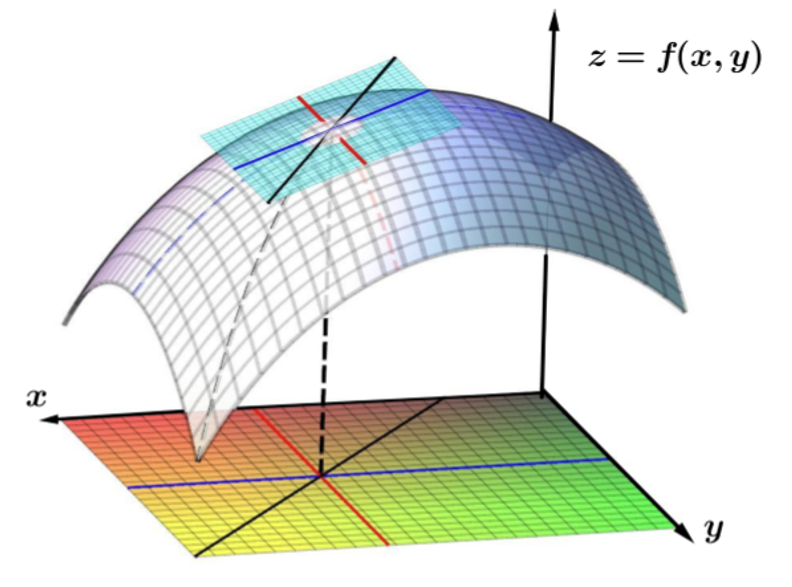
\includegraphics[width = 0.5 \textwidth]{media/GraphTangentialebene.png}
\end{center}

\begin{bsp}
	{Lineare Ersatzfunktion}{}


	Gegeben sei die Funktion
	\[
		f(x, y) = x^2 - y^2
	\]
	Gesucht ist die \textbf{lineare Ersatzfunktion} von \( f \) an der Stelle \( (1, -2) \). (Wird in der Klasse ergänzt.)

	% Die partiellen Ableitungen lauten:
	% \[
	% \frac{\partial f}{\partial x}(x, y) = 2x, \quad
	% \frac{\partial f}{\partial y}(x, y) = -2y
	% \]

	% Somit gilt:
	% \[
	% \frac{\partial f}{\partial x}(1, -2) = 2, \quad
	% \frac{\partial f}{\partial y}(1, -2) = 4
	% \]

	% Ausserdem berechnet man:
	% \[
	% f(1, -2) = 1^2 - (-2)^2 = 1 - 4 = -3
	% \]

	% Die lineare Ersatzfunktion \( T_{(1, -2)}(x, y) \) ist daher:
	% \[
	% T_{(1, -2)}(x, y) = -3 + 2(x - 1) + 4(y + 2) = 2x + 4y + 3
	% \]
	\vspace*{8cm}
\end{bsp}

\begin{ueb}
	{}{}

	\begin{enumerate}
		\item Bestimmen Sie die lineare Ersatzfunktion an der angegebenen Stelle.
		      Zeichnen Sie anschliessend den Graphen von \( f \) und jenen der Tangentialebene mit GeoGebra.
		      \begin{enumerate}
			      \item \( f(x, y) = \sqrt{x} + \sqrt{y} \), \quad \( P = (1, 1) \)
			      \item \( f(x, y) = \sqrt{xy - 1} \), \quad \( P = (5, 1) \)
			      \item \( f(x, y) = (x^2 - y^2) \cdot \sin(y) \), \quad \( P = (3, \frac{\pi}{2}) \)
		      \end{enumerate}

		\item Bestimmen Sie Näherungswerte für die folgenden Zahlen,
		      indem Sie die Funktion \( r(x, y) = \sqrt{x^2 + y^2} \) durch ihre lineare Ersatzfunktion an der Stelle \( P = (3, 4) \) approximieren:
		      \begin{enumerate}
			      \item \( \alpha = \sqrt{3.03^2 + 3.95^2} \)
			      \item \( \beta = \sqrt{2.94^2 + 4.07^2} \)
		      \end{enumerate}

		\item Geben Sie eine Gleichung der Tangentialebene an den Graphen von
		      \( f(x, y) = x^2 y^3 \) im Punkt \( P = (1 , -1) \) an.
		      Zeichnen Sie anschliessend den Graphen von \( f \) und die Tangentialebene mit GeoGebra.

		      % \item \textbf{Falls Sie die Ebenengleichung schon kennen:}  
		      % Geben Sie eine Formel für den Normalvektor der Tangentialebene an den Graphen der Funktion \( f(x, y) \) im Punkt \( P = (x_0, y_0) \) an.
	\end{enumerate}

\end{ueb}
\pagebreak
\emph{Lösungen}

\begin{enumerate}
	\item Lineare Ersatzfunktionen:
	      \begin{enumerate}
		      \item \( T_{(1,1)}(x, y) = \frac{1}{2}x + \frac{1}{2}y + 1 \)
		      \item \( T_{(5,1)}(x, y) = \frac{1}{4}x + \frac{5}{4}y - \frac{1}{2} \)
		      \item \( T_{\left(3, \frac{\pi}{2}\right)}(x, y) = 6x - \pi y + \frac{\pi^2}{4} - 9 \)
	      \end{enumerate}

	\item Näherung mit linearer Ersatzfunktion an \( P = (3,4) \) für \( r(x, y) = \sqrt{x^2 + y^2} \):
	      \[
		      T_{(3,4)}(x, y) = \frac{3}{5}x + \frac{4}{5}y
	      \]
	      \[
		      \alpha \approx 4.97, \quad \beta \approx 5.02
	      \]

	\item Tangentialebene:
	      \[
		      z = -2x + 3y + 4
	      \]

	      % \item Normalenvektor an den Graphen \( z = f(x, y) \) im Punkt \( (x_0, y_0) \):
	      % \[
	      % \vec{n} =
	      % \begin{pmatrix}
	      % f_x(x_0, y_0) \\
	      % f_y(x_0, y_0) \\
	      % -1
	      % \end{pmatrix}
	      % \]
\end{enumerate}















\clearpage
\subsection{Gradient und Richtungsableitung}
% \subsubsection*{Definition ACHTUNG: EHER WEGLASSEN (bereits halb begonnen ... )}

Genauso wie die Ableitungen in Richtung der Koordinatenachsen lassen sich natürlich auch die \emph{Richtungsableitungen} in beliebige andere Richtungen bilden.

% \begin{center}
%   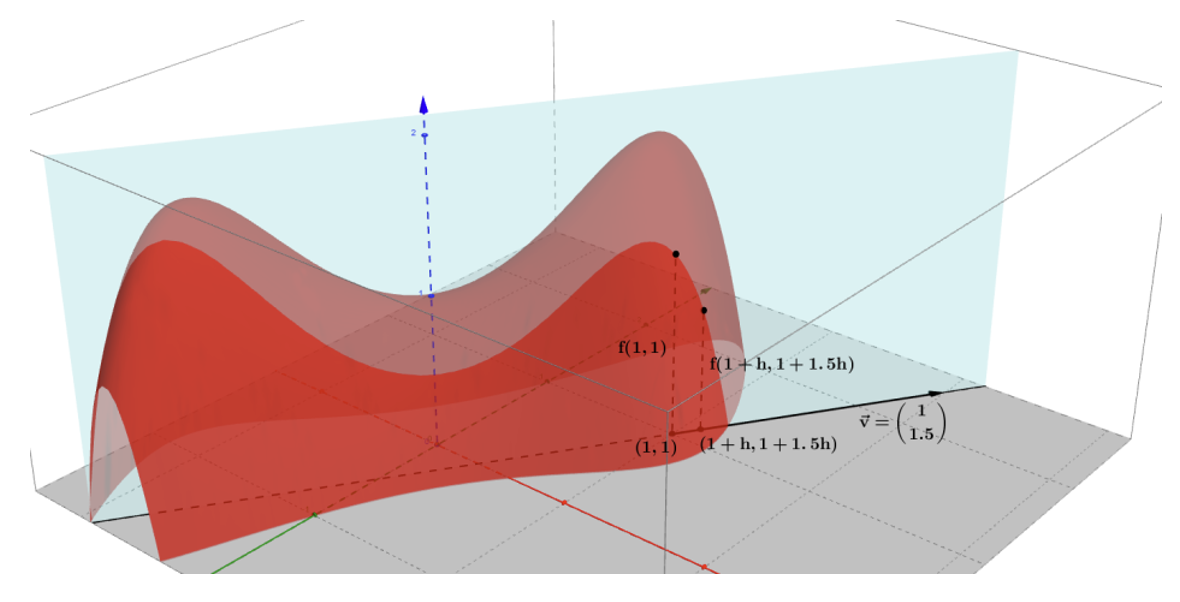
\includegraphics[width = \textwidth]{media/IntroRichtungsableitung.png}
% \end{center}

% Betrachten wir erneut den Wanderer im Punkt \( P = (1, 1) \). Diesmal läuft er jedoch in Richtung des Vektors
% \[
% \vec{v} = \begin{pmatrix} 1 \\ 1.5 \end{pmatrix}.
% \]

% Die Steigung des Weges in dieser Richtung ist gegeben durch den Grenzwert:
% \[
% \lim_{h \to 0} \frac{f(1 + h,\, 1 + 1.5h) - f(1, 1)}{\sqrt{h^2 + (1.5h)^2}}
% % =
% % \frac{1}{\sqrt{1^2 + (1.5)^2}}
% % \lim_{h \to 0} \frac{f(1 + h,\, 1 + 1.5h) - f(1, 1)}{h}
% =
% \frac{1}{|\vec{v}|}
% \lim_{h \to 0} \frac{f((1,\, 1) + h\cdot \vec{v} ) - f(1, 1)}{h}
% \]

% Dieser Ausdruck beschreibt die \textbf{Richtungsableitung} von \( f \) im Punkt \( (1, 1) \) in Richtung des Vektors \( \vec{v} \).

\begin{definition}
	{Richtungsableitung}{}

	Die Richtungsableitung einer Funktion \( f \) in Richtung eines Vektors $\vec{v}$
	% \[
	% \vec{v} = \begin{pmatrix} v_1 \\ v_2 \end{pmatrix}
	% \]
	an der Stelle \( P = (x_0, y_0) \) bezeichnet man mit
	\[ \frac{\partial f}{\partial \vec{v}}(x_0, y_0) \]
	% \[
	% \nabla_{\vec{v}} f(x_0, y_0).
	% \]
	% 

	Sie ist definiert durch den Grenzwert:
	\[
		%\nabla_{\vec{v}} f(x_0, y_0)
		\frac{\partial f}{\partial \vec{v}}(x_0, y_0)
		=
		\lim_{h \to 0}
		\frac{
			f((x_0 ,\, y_0) + h \vec{v}) - f(x_0, y_0)
			% =
			% \lim_{h \to 0}
			% \frac{
			% f(x_0 + h v_1,\, y_0 + h v_2) - f(x_0, y_0)
		}{
			h
		}
	\]

\end{definition}

\textbf{Bemerkungen:}
\begin{itemize}
	\item Die Richtungsableitung beschreibt die Steigung der Schnittkurve, die man erhält, wenn man den Graphen von \( f \) mit einer Ebene schneidet, die durch den Punkt \( P = (x_0, y_0, f(x_0, y_0)) \) verläuft und die Richtung des Vektors \( \vec{v} \) enthält.
	\item Man beachte jedoch, dass die horizontalen Änderung in Vielfache von $|\vec{v}|$ gemessen wird. Darum ist die Richtungsableitung vom Betrag des Vektors $\vec{v}$ abhängig. Die Richtungsableitung einer Funktion $f$ in Richtung des Vektors $2\cdot\vec{v}$ wird doppelt so gross sein, wie jene in Richtung des Vektors $\vec{v}$.
	\item Aus diesem Grund wird die Richtungsableitung häufig nur für normierte Vektoren, also für Vektoren der Länge Eins, betrachtet. In diesem Fall ist die Richtungsableitung tatsächlich eine Steigung.
	\item Die Richtungsableitung ist eine Verallgemeinerung der partiellen Ableitungen. Denn die Richtungsableitung in Richtung des Vektors \( \begin{pmatrix} 1 \\ 0 \end{pmatrix} \) entspricht der partiellen Ableitung nach \( x \), und die Richtungsableitung in Richtung des Vektors \( \begin{pmatrix} 0 \\ 1 \end{pmatrix} \) entspricht der partiellen Ableitung nach \( y \).
\end{itemize}






% \begin{satz}
% {Richtungsableitung und Steigung der Schnittkurve}{}
% Sei $f$ eine Funktion $f:\R^2\to\R^2$, $(x_0, y_0)\in \DD_f$  und $\vec{v} \in \R^2$. 

% \end{satz}

% \begin{bsp}
% 	{}{RichtungsableitungGrenzwert}
% 	Gegeben sei die Funktion
% 	\[
% 		f(x, y) = e^{xy}
% 	\]
% 	und der Punkt \( P = (1, 1) \). Gesucht ist die Richtungsableitung von \( f \) in Richtung des Vektors
% 	\[
% 		\vec{v} = \begin{pmatrix} 1 \\ 2 \end{pmatrix}.
% 	\]

% 	\vspace*{15cm}
% \end{bsp}

% \clearpage
\subsubsection*{Zusammenhang mit der partiellen Ableitung}
Die Ermittlung der Richtungsableitung mit dem Grenzwert kann sehr aufwendig sein. Abhilfe schafft eine geometrische Überlegung. Betrachten Sie die folgende Grafik
\begin{center}
	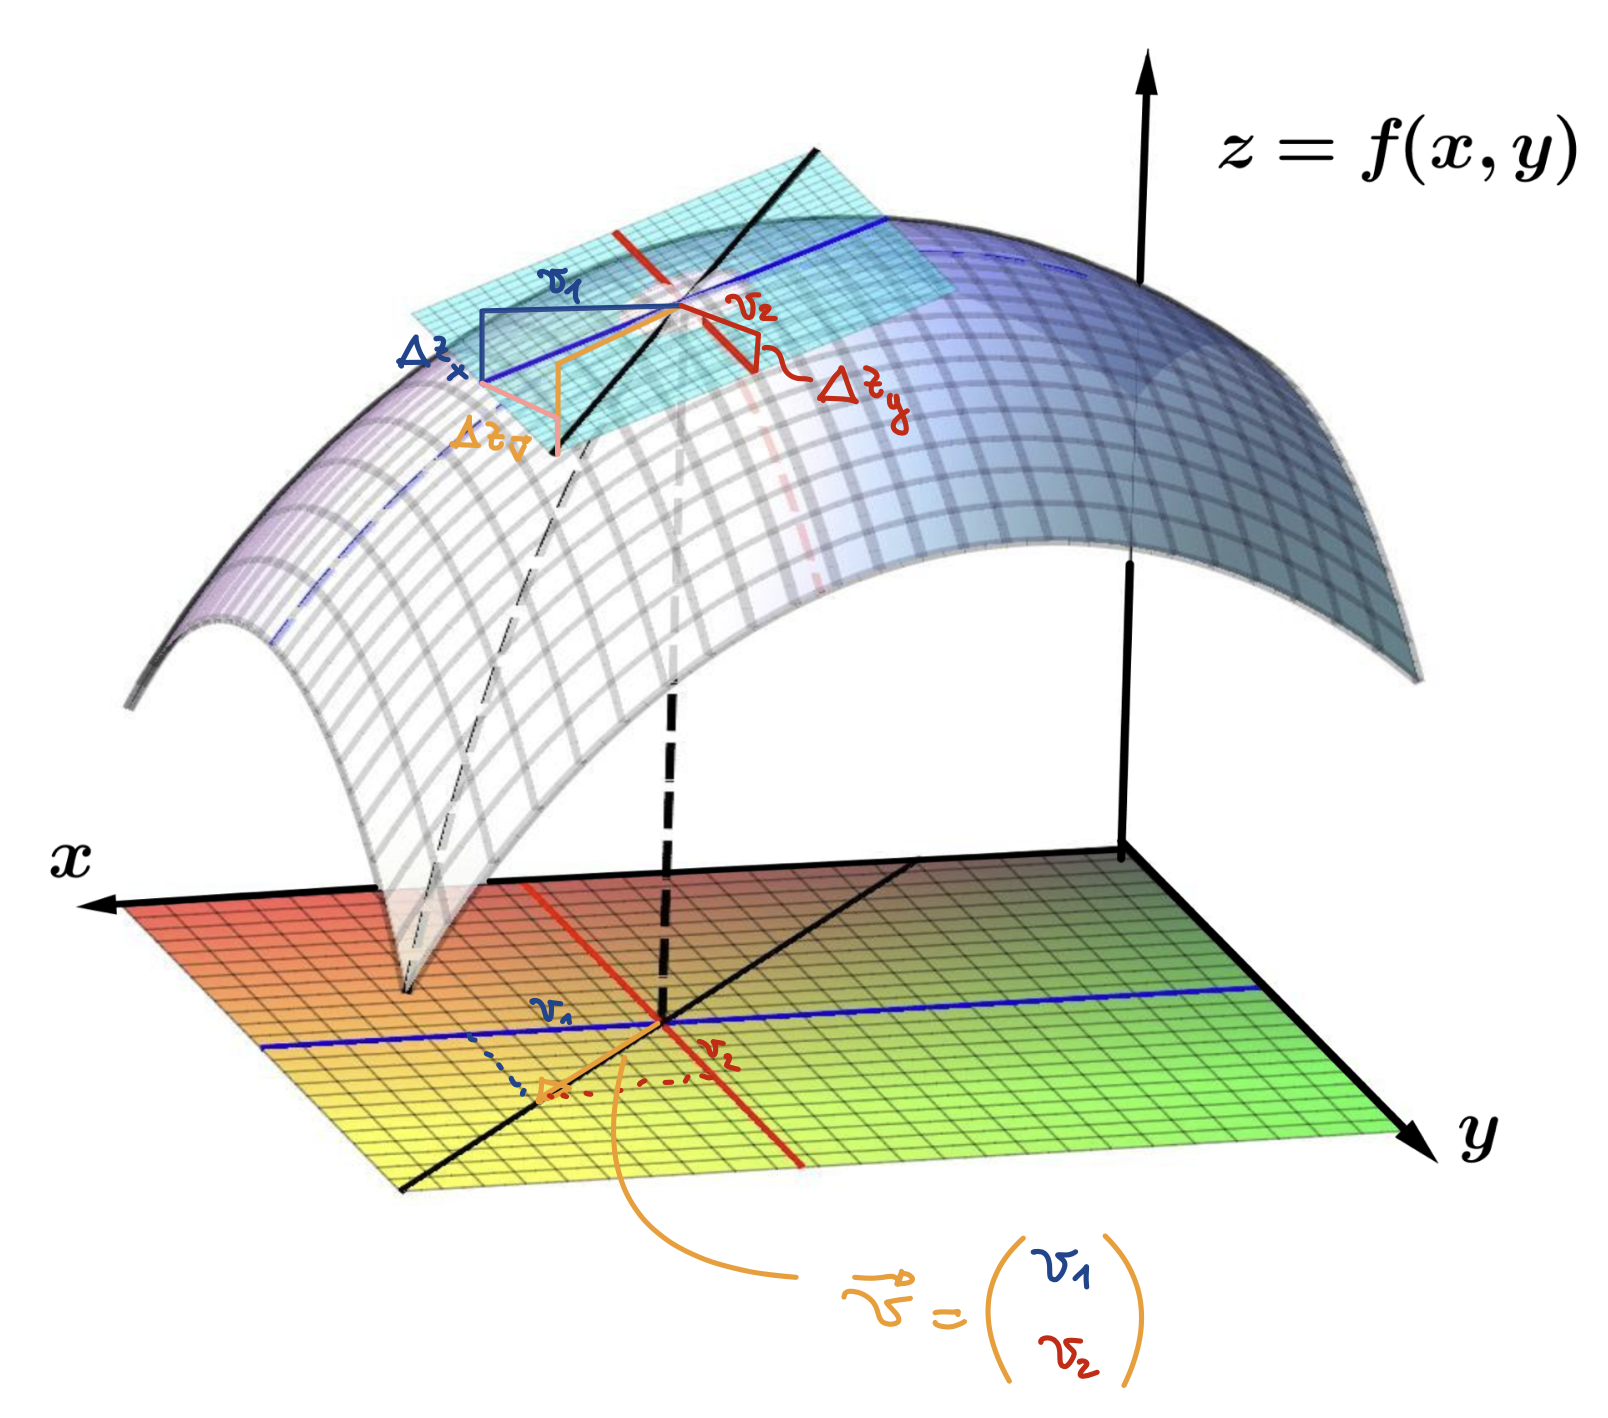
\includegraphics[width = \textwidth]{media/GradientundpartielleAbleitung.png}
\end{center}
Die Richtngsableitung $\frac{\partial f}{\partial \vec{v}}(x_0, y_0)$ ist die lokale Änderung der $z$-Koordinate, wenn man sich vom Punkt $(x_0, y_0)$ in Richtung des Vektors $\vec{v}$ bewegt. Mit den Bezeichnungen in der Grafik ist also:

\[
	%\nabla_{\vec{v}} f(x, y)
	\frac{\partial f}{\partial \vec{v}}(x_0, y_0)  = \Delta z_{\vec{v}}
\]

Für die Änderungen entlang der Koordinatenrichtungen gilt:

\[
	% \frac{\partial f}{\partial x}(x, y) = \frac{\Delta z_x}{v_1}
	% \quad \Rightarrow \quad
	\Delta z_x = v_1 \cdot \frac{\partial f}{\partial x}(x, y)
\]

\[
	% \frac{\partial f}{\partial y}(x, y) = \frac{\Delta z_y}{v_2}
	% \quad \Rightarrow \quad
	\Delta z_y = v_2 \cdot \frac{\partial f}{\partial y}(x, y)
\]

Offensichtlich gilt:
\[
	\Delta z_{\vec{v}} = \Delta z_x + \Delta z_y =
	v_1 \cdot \frac{\partial f}{\partial x}(x, y) +
	v_2 \cdot \frac{\partial f}{\partial y}(x, y)
\]

\begin{center}
	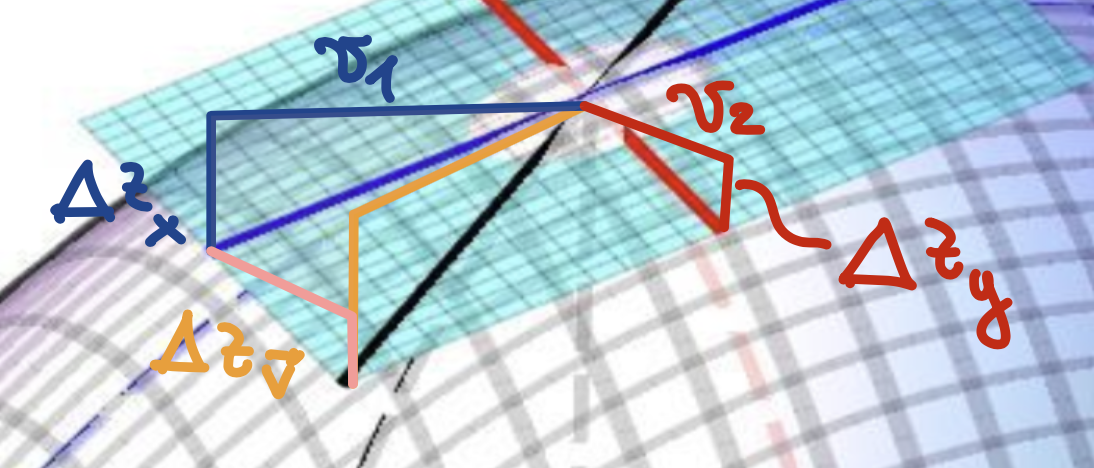
\includegraphics[width = \textwidth]{media/gradientundpartielleAbleitung2.png}
\end{center}

\begin{satz}
	{Richtungsableitung aus den partiellen Ableitungen}{}
	Es sei \( f \) eine stetig differenzierbare Funktion in zwei Variablen,
	sei \( (x_0, y_0) \) ein Punkt des Definitionsbereichs von \( f \),
	und sei
	\[
		\vec{v} = \begin{pmatrix} v_1 \\ v_2 \end{pmatrix}
	\]
	ein beliebiger Richtungsvektor.

	Dann gilt für die Richtungsableitung von \( f \) in Richtung \( \vec{v} \) an der Stelle \( (x_0, y_0) \):
	\[
		%\nabla_{\vec{v}} f(x_0, y_0) 
		\frac{\partial f}{\partial \vec{v}}(x_0, y_0) =
		v_1 \cdot \frac{\partial f}{\partial x}(x_0, y_0)
		+ v_2 \cdot \frac{\partial f}{\partial y}(x_0, y_0)
	\]
\end{satz}

Mit diesem Satz lässt sich die Richtungsableitung einfach berechnen.

\begin{bsp}
	{}{}
	% Vergleiche \Cref{bsp:RichtungsableitungGrenzwert}:
	Gegeben sei die Funktion
	\[
		f(x, y) = e^{xy}
	\]
	und der Punkt \( P = (1, 1) \). Gesucht ist die Richtungsableitung von \( f \) in Richtung des Vektors
	\[
		\vec{v} = \begin{pmatrix} 1 \\ 2 \end{pmatrix}.
	\]
	\vspace*{5cm}
\end{bsp}

\begin{ueb}
	{}{}


	\begin{enumerate}
		\item Berechnen Sie die Richtungsableitung der Funktion
		      \[
			      f(x, y) = 100xy
		      \]
		      in Richtung des Vektors
		      \[
			      \vec{v} = \begin{pmatrix} 1 \\ -1 \end{pmatrix}
		      \]
		      an der Stelle \( P = (x_0, y_0) \).

		\item \textbf{Kegel:}
		      \begin{enumerate}
			      \item

			            Berechnen Sie die Richtungsableitung der Funktion
			            \[
				            f(x, y) = \sqrt{x^2 + y^2}
			            \]
			            in Richtung des Vektors
			            \[
				            \vec{v} = \frac{1}{5} \begin{pmatrix} 4 \\ 3 \end{pmatrix}
			            \]
			            an der Stelle \( P = (x_0, y_0) \).



			      \item Liefern Sie eine \textbf{geometrische Erklärung} für die folgenden Aussagen zur Richtungsableitung aus Aufgabe (a).
			            (Es ist hilfreich, den Graphen mit GeoGebra darzustellen)

			            \begin{enumerate}
				            \item Die Richtungsableitung an der Stelle \( P = (0, 0) \) existiert nicht.
				            \item Die Richtungsableitung an der Stelle \( P = (4, 3) \) ist gleich Eins.
				            \item Die Richtungsableitung an der Stelle \( P = (-3, 4) \) ist gleich Null.
			            \end{enumerate}
		      \end{enumerate}
	\end{enumerate}

\end{ueb}

\clearpage
\emph{Lösungen}
\begin{enumerate}
	\item $100(y_0-x_0)$
	\item $\frac{4x_0+3y_0}{5\sqrt{x_0^2 + y_0^2}}$
\end{enumerate}




















\clearpage
\subsubsection*{Der Gradient}
Häufig wird der Term in der Formel für die Richtungsableitung als Skalarprodukt von zwei Vektoren interpretiert. Das Skalarprodukt wird im Grundlagenfach Mathematik behandeln. Für unsere Zwecke übernehmen wir ein paar Fakten, die im Grundlagenfach bewiesen werden.

Physikalische Grössen wie etwa Kraft, Geschwindigkeit oder Impuls beinhalten eine Richtung und werden mit Vektoren beschrieben, während Grössen wie Masse, Zeit oder Temperatur ungerichtet sind und sich durch eine einzige Zahl angeben lassen, die man in der Physik als Skalar bezeichnet.

\begin{definition}
	{Skalarprodukt}{}
	Seien $\vec{a}=\begin{pmatrix}
			a_1 \\a_2
		\end{pmatrix}$ und $\vec{b} = \begin{pmatrix}
			b_1 \\b_2
		\end{pmatrix}$ zwei Vektoren in $\R^2$. Dann ist das Skalarprodukt $\langle \vec{a}, \vec{b} \rangle$  definiert als
	$$ \langle \vec{a}, \vec{b} \rangle = a_1b_1 + a_2b_2$$
\end{definition}

\begin{bsp}
	{}{}
	$$\left\langle \begin{pmatrix} -2 \\ 3 \end{pmatrix}
		,
		\begin{pmatrix} 4 \\ 1 \end{pmatrix}
		\right\rangle
		= (-2) \cdot 4 + 3 \cdot 1
		= -8 + 3 = -5 $$
\end{bsp}

\textbf{Bemerkungen:}

\begin{itemize}
	\item Im Grundlagenfach bezeichnen wir das Skalarprodukt eher mit $\vec{a}\cdot \vec{b}$. Im Schwerpunktfach verwenden wir hingegen diese Notation, die auch an Hochschulen üblich ist.
	\item \( \vec{a} \) und \( \vec{b} \) sind Vektoren (sie haben eine Richtung),
	      \( \langle \vec{a}, \vec{b} \rangle \) ist ein \emph{Skalar} – also „bloss eine Zahl“.


	\item Seien \( \vec{a} \) und \( \vec{b} \) zwei Vektoren mit den Längen \( |\vec{a}| = 4 \) und \( |\vec{b}| = 3 \).
	      Je nach Zwischenwinkel \( \varepsilon \) variiert der Wert des Skalarprodukts \( \langle \vec{a}, \vec{b} \rangle \) wie folgt:

	      \begin{center}
		      \begin{tabular}{c|ccccccc}
			      \( \varepsilon \)                      & \( 0^\circ \) & \( 30^\circ \)  & \( 60^\circ \) & \( 90^\circ \) & \( 120^\circ \) & \( 150^\circ \)  & \( 180^\circ \) \\
			      \hline
			      \( \langle \vec{a}, \vec{b} \rangle \) & $12$          & \( 6\sqrt{3} \) & $6$            & $0$            & $-6$            & \( -6\sqrt{3} \) & $-12$
		      \end{tabular}
	      \end{center}



	      Der Wert des Skalarprodukts gibt also gewissermassen an, wie die beiden Vektoren zueinanderstehen.

\end{itemize}

Der Zusammenhang zwischen Skalarprodukt und gegenseitige Lage der Vektoren wird im Grundlagenfach genauer behandelt. Hier werden wir bloss zwei Fakten festhalten, die wir noch brauchen werden:
\clearpage
\begin{satz}
	{Skalarprodukt und gegenseitige Lage}{SkalarproduktundgegeseitigeLage}
	Für zwei Vektoren $\vec{a}$ und $\vec{b}$ gilt

	\begin{itemize}
		\item $ \vec{a}$ und $\vec{b}$ stehen genau dann senkrecht aufeinander, wenn deren Skalarprodukt $0$ ist:
		      $$ \vec{a} \perp \vec{b} \iff \langle\vec{a}, \vec{b} \rangle = 0$$
		\item Das Skalarprodukt von zwei Vektoren mit fester Länge ist genau dann maximal, wenn die Vektoren in die gleiche Richtung zeigen. In diesem Fall gilt
		      $$\vec{a} = \lambda\cdot \vec{b} \quad (\lambda >0)  \iff \langle\vec{a}, \vec{b} \rangle  = |\vec{a}| \cdot |\vec{b}|$$
	\end{itemize}

\end{satz}

\begin{bsp}
	{}{}
	\[
		\left\langle
		\begin{pmatrix} -2 \\ 3 \end{pmatrix},
		\begin{pmatrix} 6 \\ 4 \end{pmatrix}
		\right\rangle
		= (-2) \cdot 6 + 3 \cdot 4 = -12 + 12 = 0
	\]

	Die beiden Vektoren stehen  \textbf{senkrecht} aufeinander!

\end{bsp}

Mit dem Skalarprodukt lässt sich die Richtungsableitungen elegant berechnen. Es gilt nämlich:
\[
	%\nabla_{\vec{v}} f(x_0, y_0)
	\frac{\partial f}{\partial \vec{v}}(x_0, y_0)=
	v_1 \cdot \frac{\partial f}{\partial x}(x_0, y_0)
	+ v_2 \cdot \frac{\partial f}{\partial y}(x_0, y_0)
	= \left\langle \begin{pmatrix}
		\frac{\partial f}{\partial x}(x_0, y_0) \\
		\frac{\partial f}{\partial y}(x_0, y_0)
	\end{pmatrix}
	,
	\begin{pmatrix}
		v_1 \\v_2
	\end{pmatrix}
	\right\rangle
	=\langle \vec{\nabla} f(x_0, y_0), \vec{v} \rangle
\]

\begin{definition}
	{Der Gradient}{}
	Sei \( f \colon \mathbb{R}^2 \to \mathbb{R} \) eine Funktion mit der Eigenschaft, dass beide partiellen Ableitungen existieren.

	Der Gradient \( \vec{\nabla} f(x_0, y_0) \) von \( f \) im Punkt \( P = (x_0, y_0) \) ist der Vektor:
	\[
		\vec{\nabla} f(x_0, y_0) =
		\begin{pmatrix}
			\frac{\partial f}{\partial x}(x_0, y_0) \\
			\frac{\partial f}{\partial y}(x_0, y_0)
		\end{pmatrix}
	\]

\end{definition}

Mit dem Gradienten lässt sich die Richtungsableitung neu wie folgt berechnen:
\begin{satz}
	{Richtungsableitung als Skalarprodukt}{}

	Es sei \( f \) eine stetig differenzierbare Funktion in zwei Variablen und
	\( (x_0, y_0) \) ein Punkt des Definitionsbereiches von \( f \). Dann gilt:

	\[
		%\nabla_{\vec{v}} f(x_0, y_0)
		\frac{\partial f}{\partial \vec{v}}(x_0, y_0) = \left\langle \vec{\nabla} f(x_0, y_0),\, \vec{v} \right\rangle
	\]

	Dabei bezeichnet \( \langle \cdot, \cdot \rangle \) das \textbf{Skalarprodukt} der beiden Vektoren.

\end{satz}

Auf den ersten Blick hat man damit nicht viel gewonnen. Die Richtungsableitung wird immer noch genau gleich berechnet. Durch die Interpretation der Formel als Skalarprodukt können wir aber die geometrischen Eigenschaften des Skalarprodukt (also \Cref{satz:SkalarproduktundgegeseitigeLage}) auf die Richtungsableitung übertragen!

\begin{satz}
	{Eigenschaften des Gradienten}{}
	Für den Gradient$\vec{\nabla} f(x_0, y_0)$ einer Funktion $f$ an der Stelle $(x_0, y_0)$ gilt:
	\begin{itemize}
		\item $\vec{\nabla} f(x_0, y_0)$ steht senkrecht zur Niveaulinie von $f$ durch $(x_0, y_0)$.
		\item Die Richtung des Gradienten $\vec{\nabla} f(x_0, y_0)$ gibt die Richtung der grössten Richtungsableitung von $f$ in $(x_0,y_0)$ an (Richtung des maximalen Anstiegs des Graphen von $f$).
	\end{itemize}
\end{satz}

\begin{proof}
	\begin{itemize}
		\item Da sich der Funktionswert entlang der Niveaulinien nicht ändert, ist die Ableitung in Richtung der Tangente gleich null.

		      Das heisst: Ist \( \vec{v} \) ein Tangentenvektor an die Niveaulinie im Punkt \( (x_0, y_0) \), dann gilt:
		      \[
			      0 =
			      %\nabla_{\vec{v}} f(x_0, y_0)
			      \frac{\partial f}{\partial \vec{v}}(x_0, y_0)
			      = \left\langle \vec{\nabla} f(x_0, y_0),\, \vec{v} \right\rangle
		      \]
		      Aus \Cref{satz:SkalarproduktundgegeseitigeLage} folgt dann, dass die beiden Vektoren $\vec{\nabla} f(x_0, y_0)$ und  $\vec{v}$ senkrecht stehen. Fazit: Der Gradient steht stets senkrecht auf den Niveaulinien.
		      % \[
		      % \Longleftrightarrow \quad \left\langle \vec{\nabla} f(x_0, y_0),\, \vec{v} \right\rangle = 0
		      % \quad \Longleftrightarrow \quad \vec{v} \perp \vec{\nabla} f(x_0, y_0)
		      % \]
		\item Betrachten man alle Vektoren $\vec{v}$ in $\R^2$ dann ist die Richtungsableitung $\frac{\partial f}{\partial \vec{v}}(x_0, y_0)
			      = \left\langle \vec{\nabla} f(x_0, y_0),\, \vec{v} \right\rangle$ genau dann maximal, wenn $\vec{v} = \lambda  \vec{\nabla} f(x_0, y_0)$ (\Cref{satz:SkalarproduktundgegeseitigeLage}).

	\end{itemize}
\end{proof}

\noindent
\begin{minipage}[t]{0.48\textwidth}
	\centering
	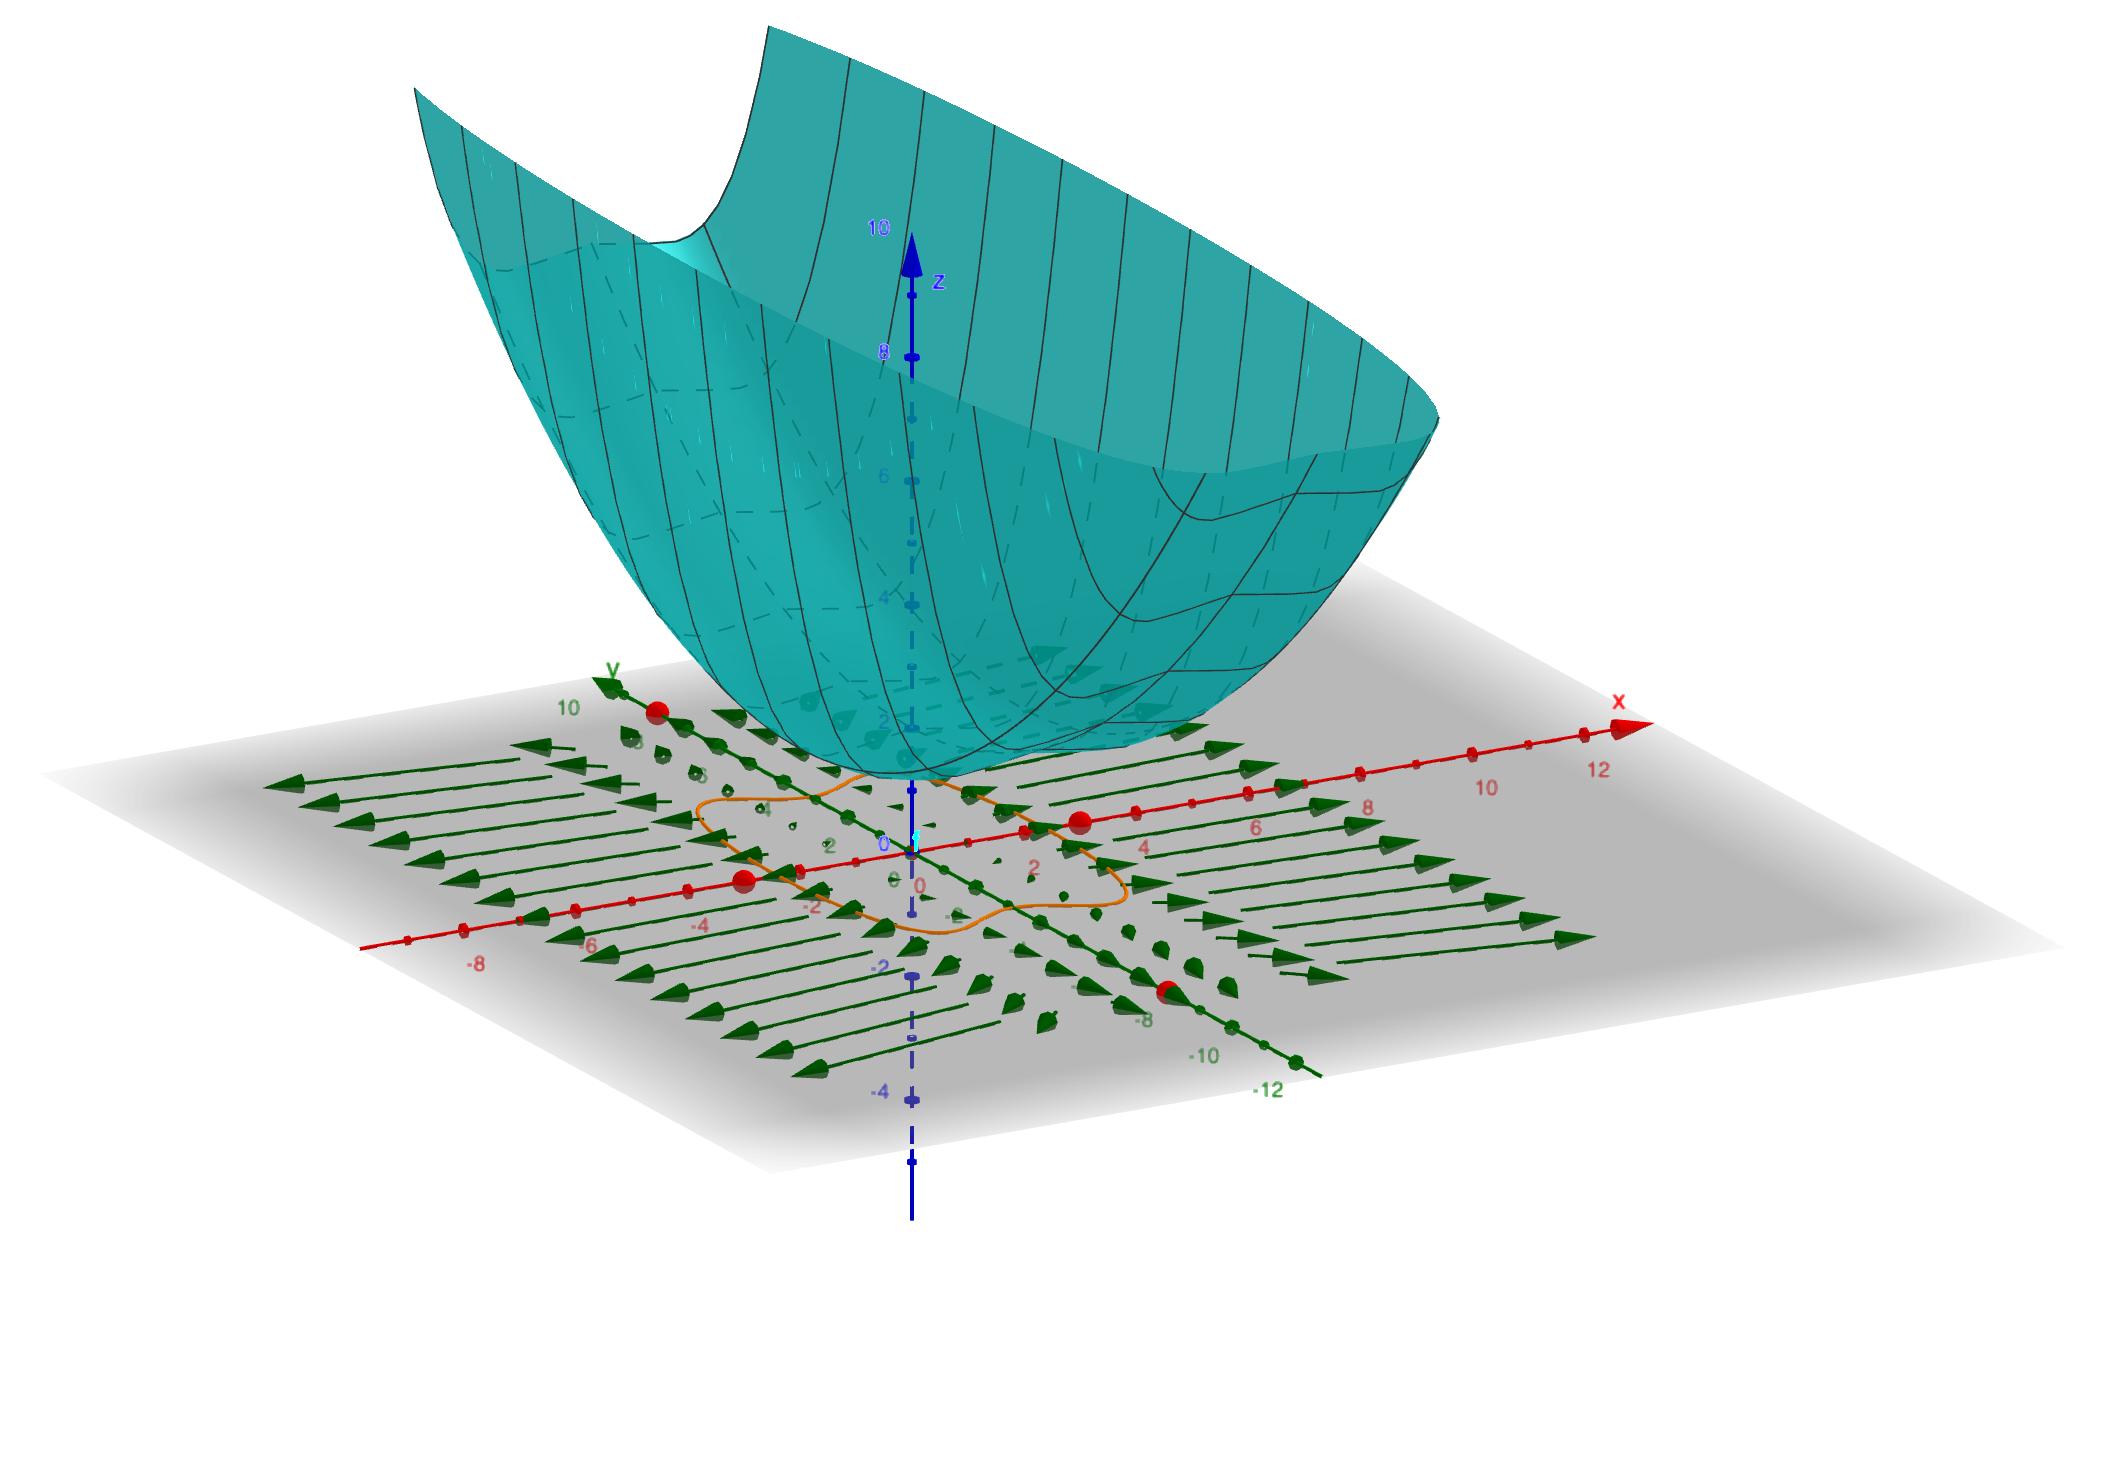
\includegraphics[width=\linewidth]{media/GradientenFeld.png}\\
	\small Graph einer Funktion $f$
\end{minipage}
\hfill
\begin{minipage}[t]{0.48\textwidth}
	\centering
	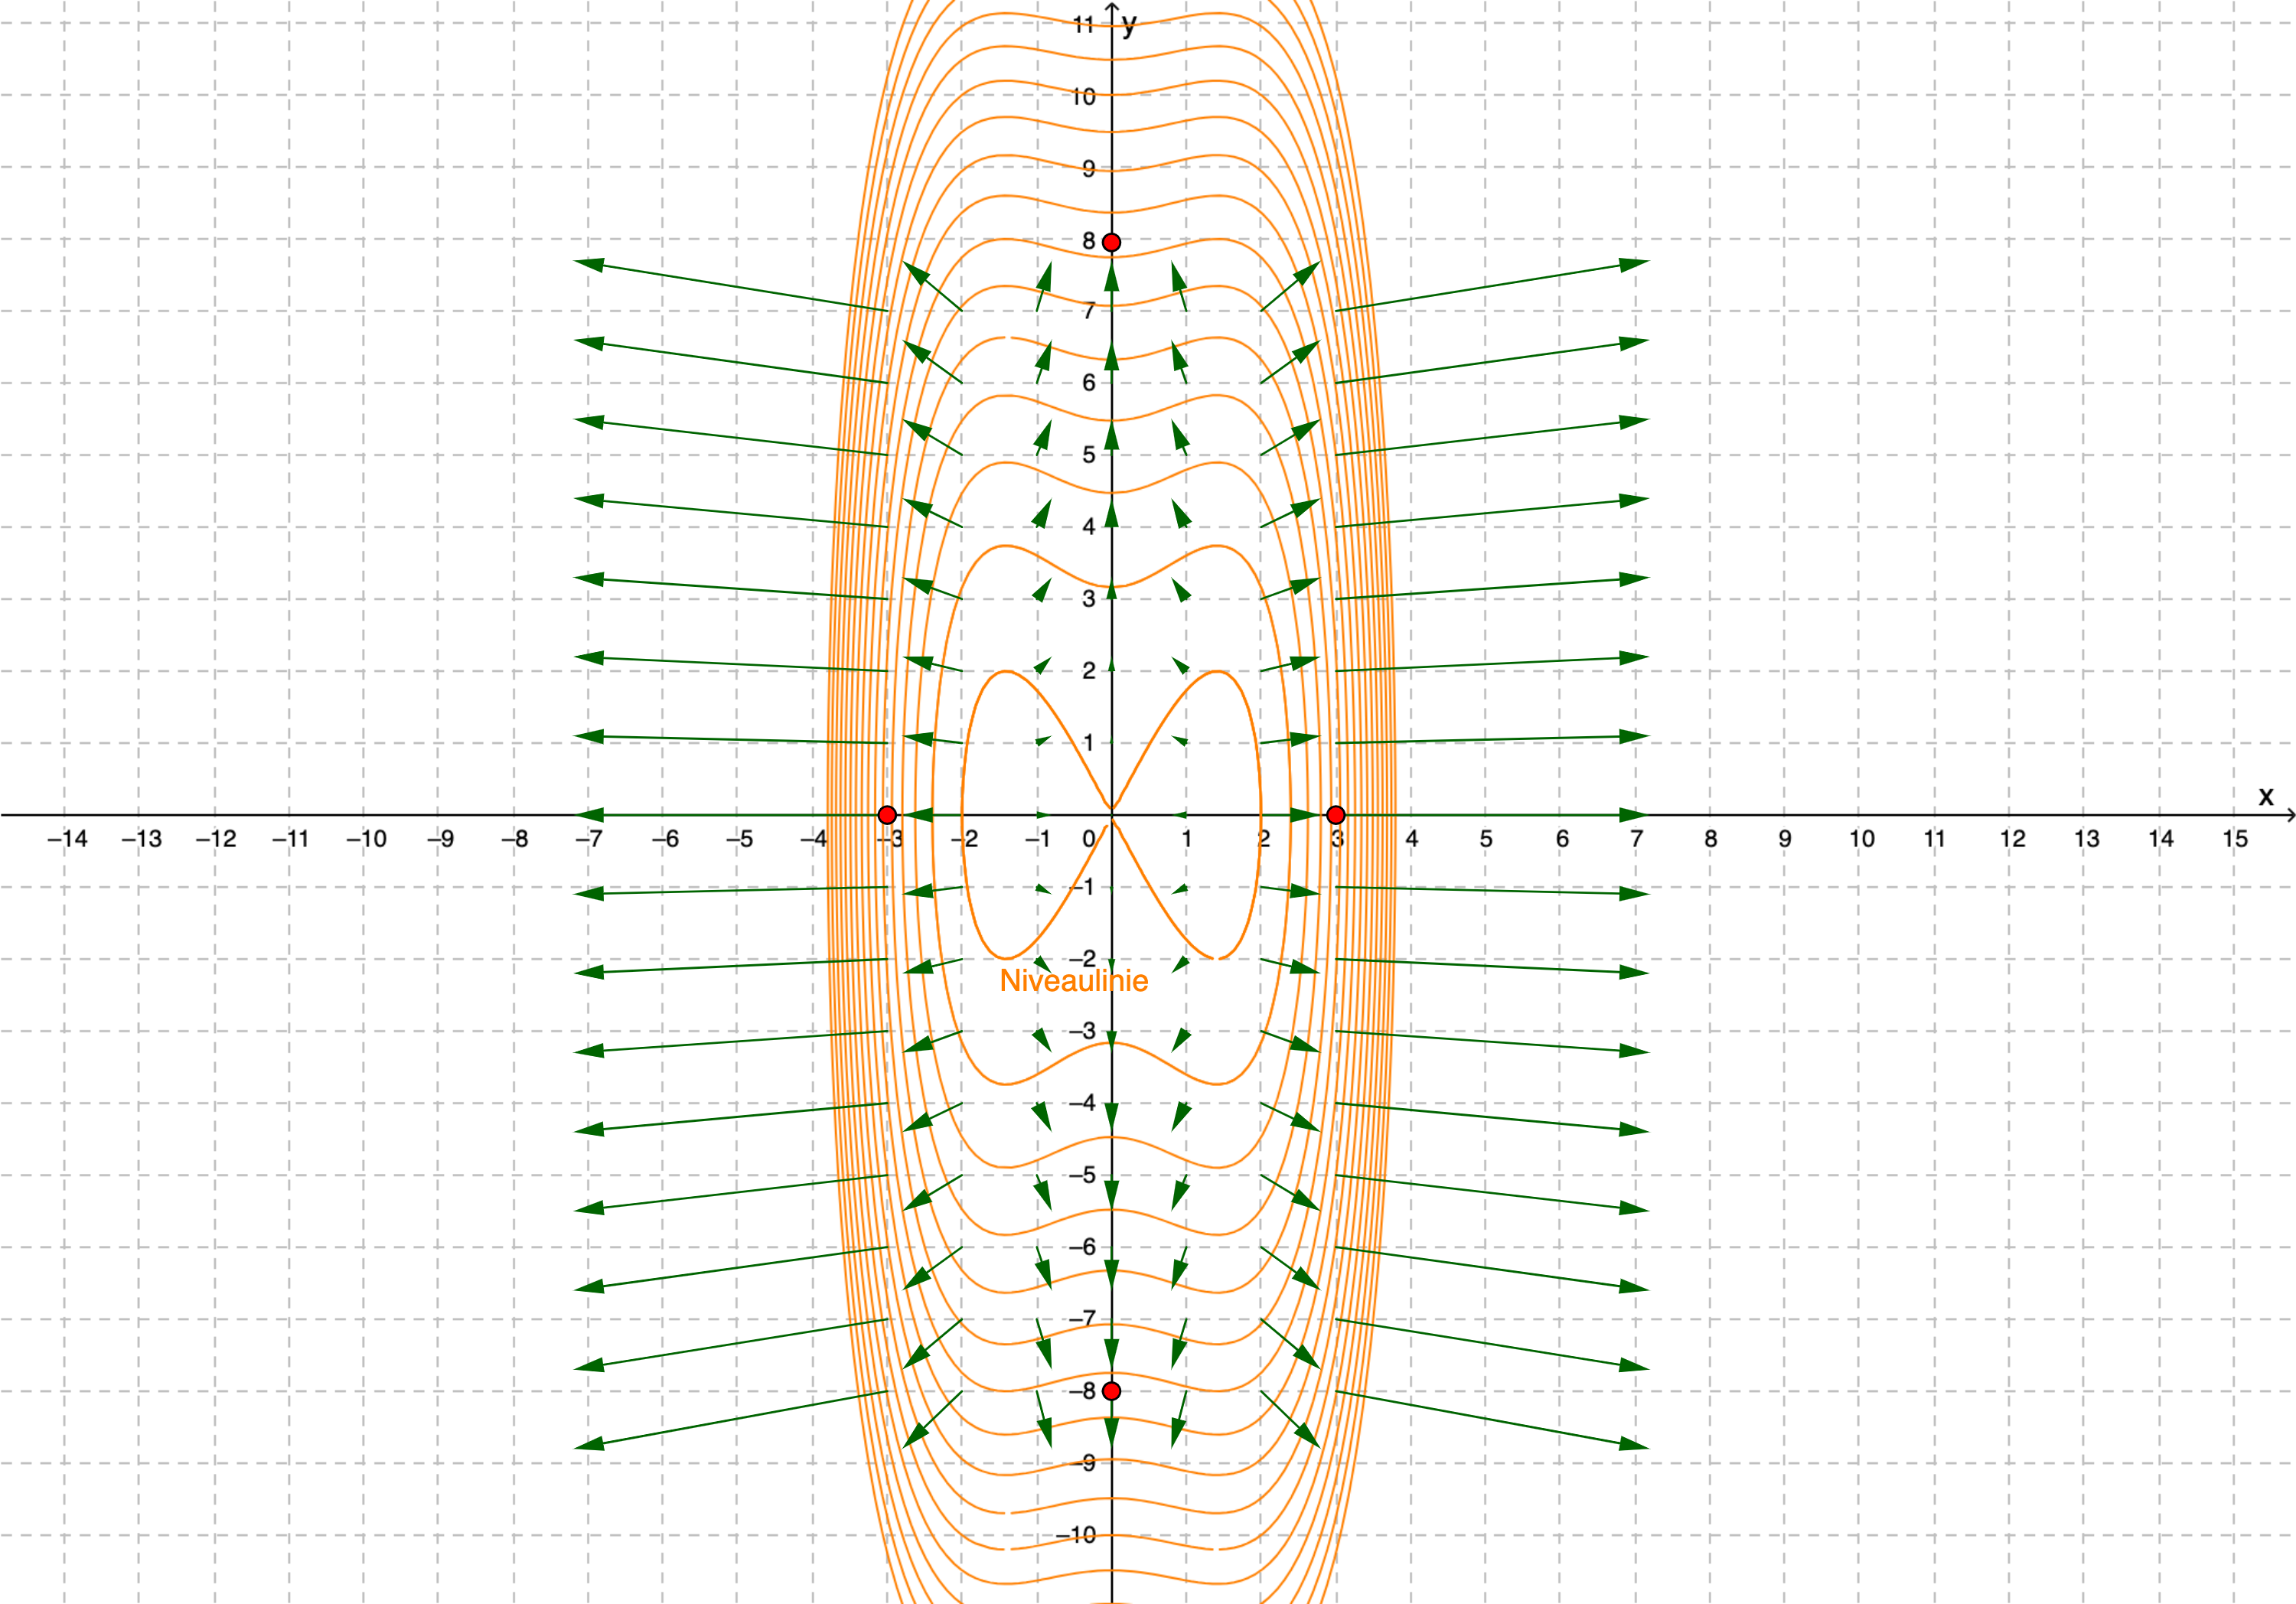
\includegraphics[width=\linewidth]{media/GradientNiveaulinie.png}\\
	\small Niveaulinien und Gradientenfeld der Funktion $f$
\end{minipage}

% \begin{center}
%   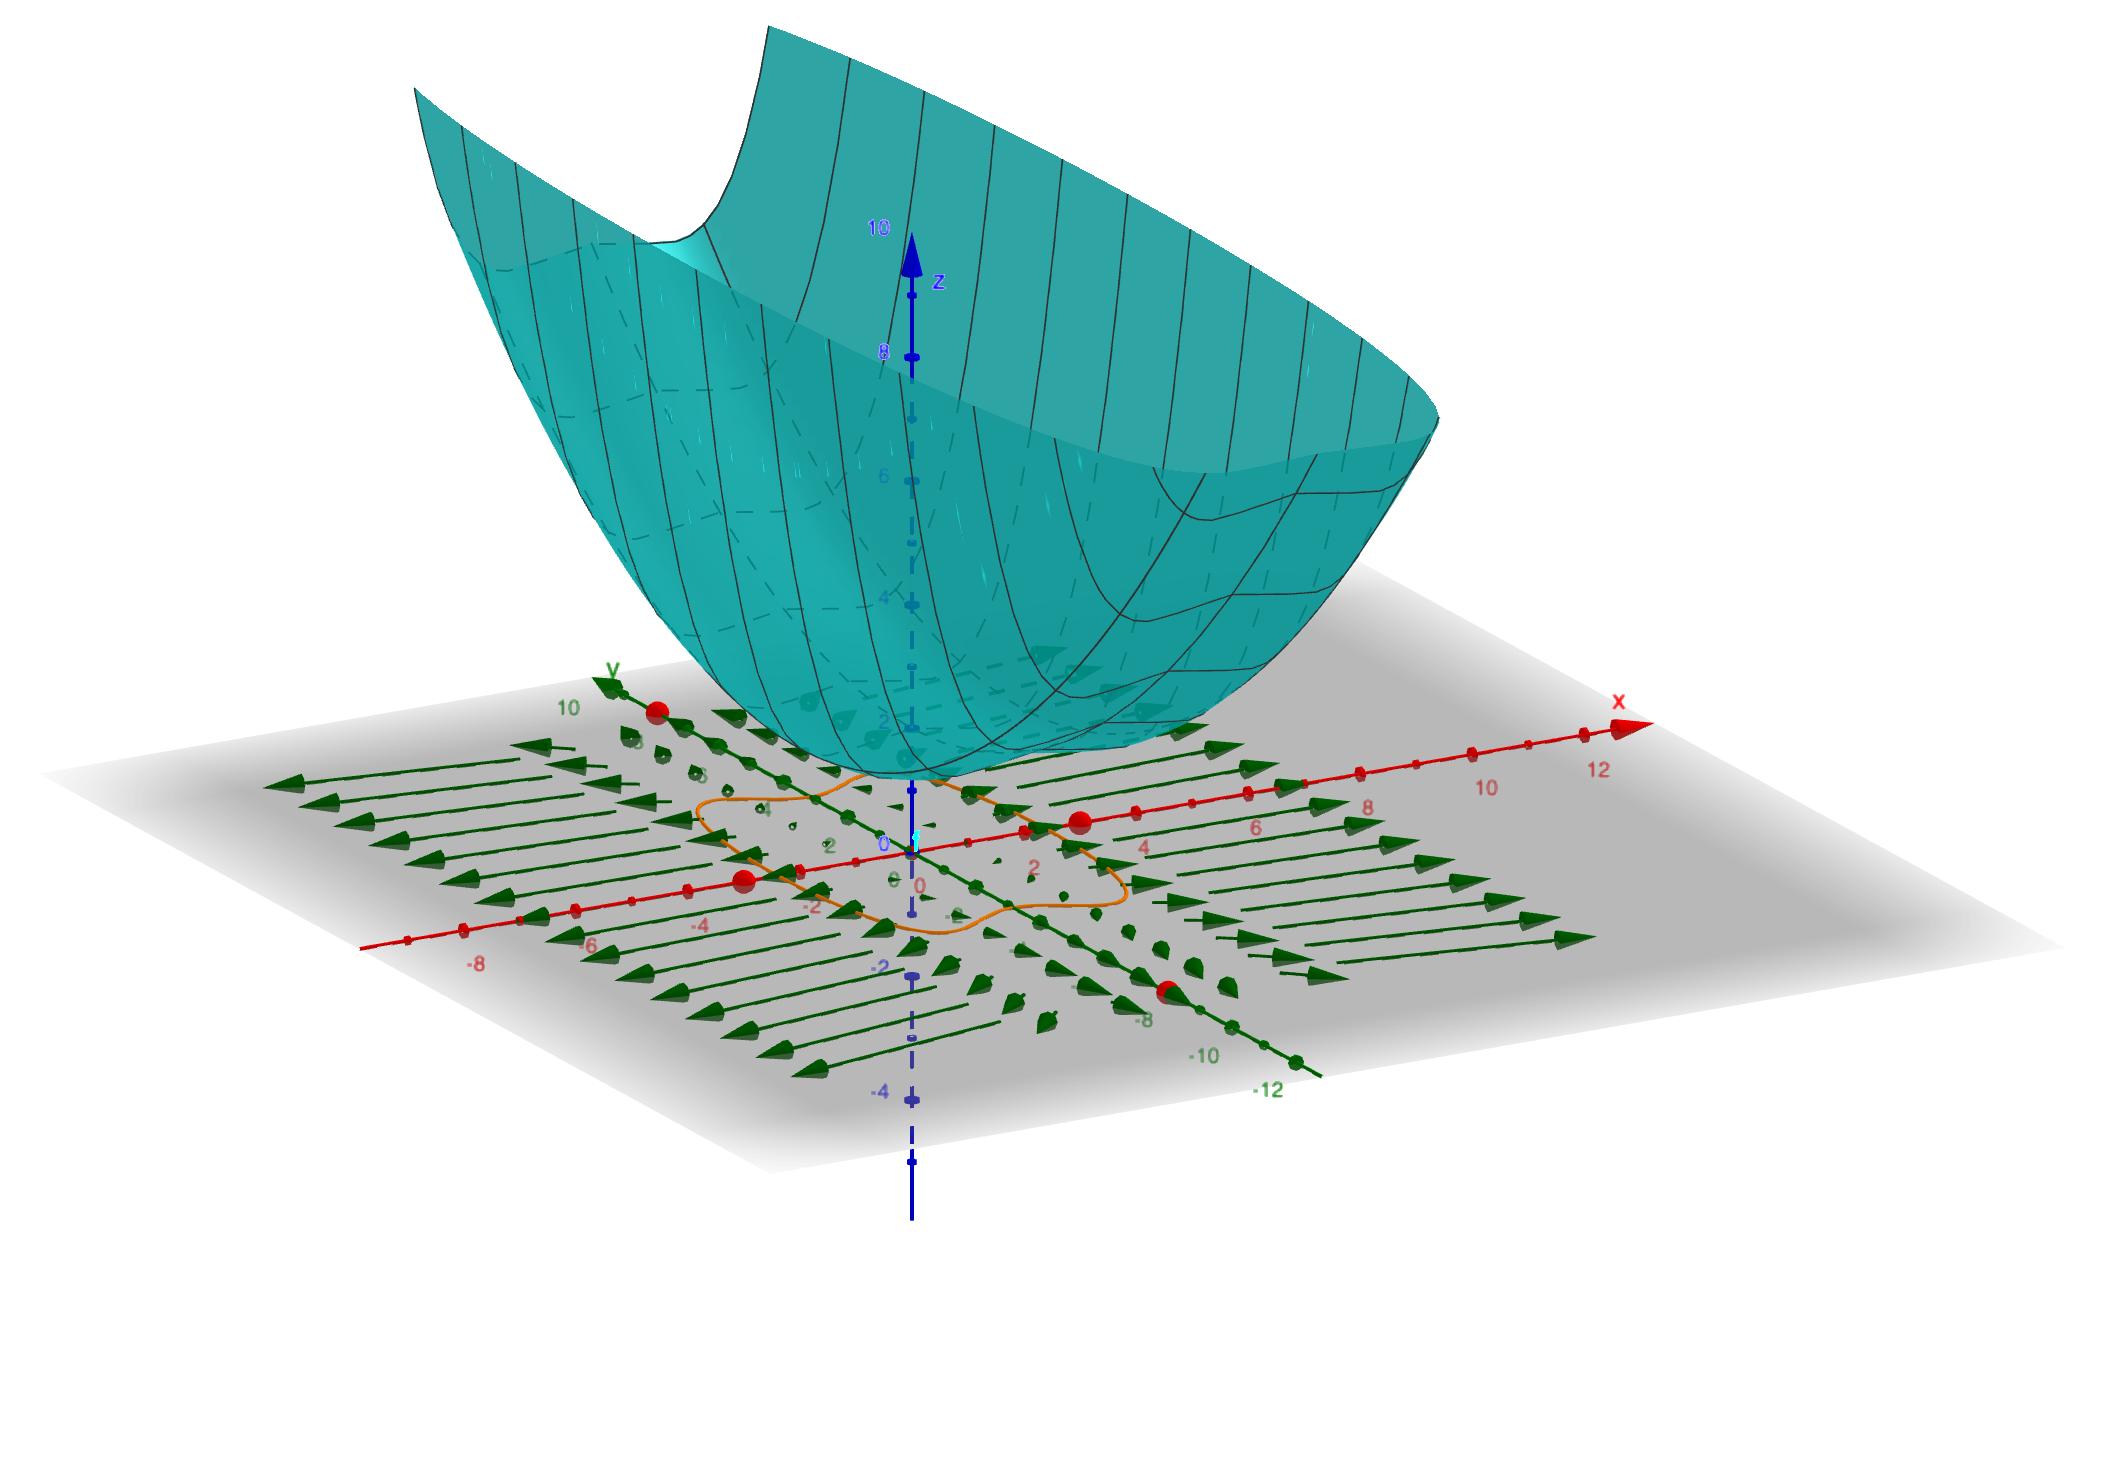
\includegraphics[width = \textwidth]{media/GradientenFeld.png}
%   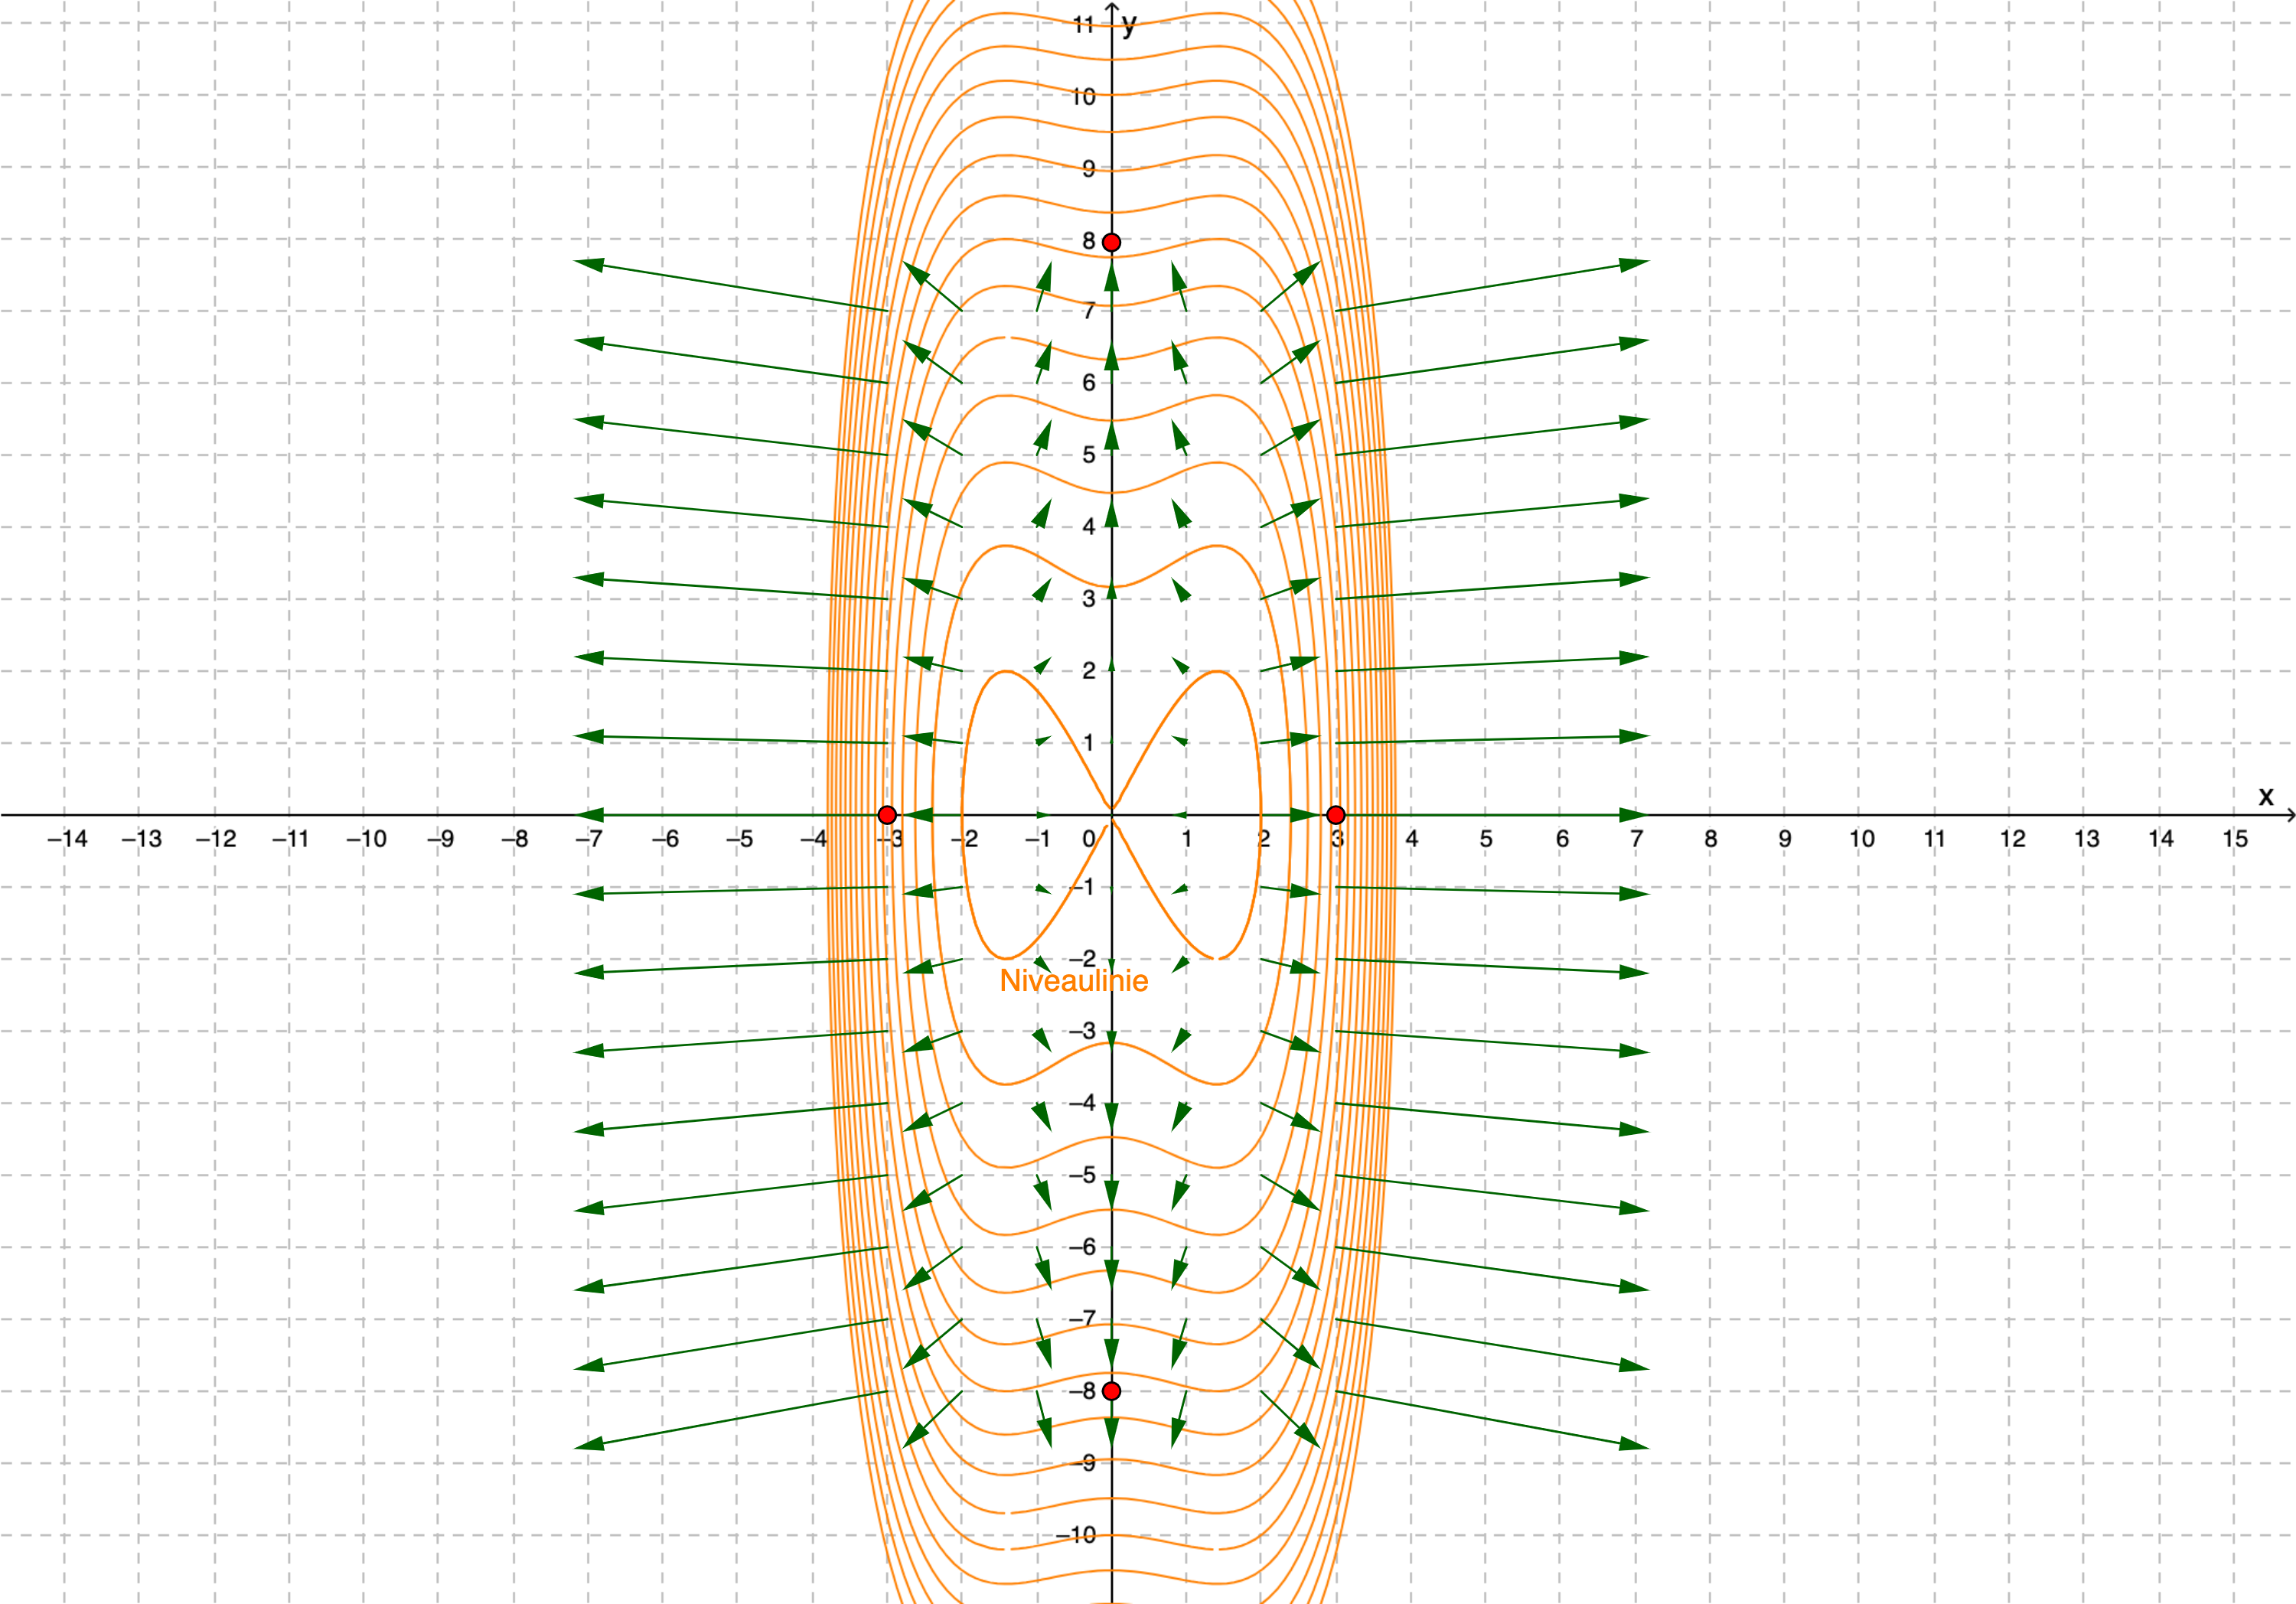
\includegraphics[width = \textwidth]{media/GradientNiveaulinie.png}

% \end{center}
\clearpage
\begin{ueb}
	{}{}

	\begin{enumerate}
		\item Gegeben ist die Funktion
		      \[
			      f(x, y) = 2x^2 y - 4xy + 3y^2.
		      \]
		      \begin{enumerate}
			      \item Bestimmen Sie den Gradienten \( \vec{\nabla} f(x, y) \).
			      \item Geben Sie die Richtungsableitung \(\frac{\partial f}{\partial \vec{v}}(2, -5) \) mit
			            \[
				            \vec{v} = \begin{pmatrix} -6 \\ 8 \end{pmatrix}
			            \]
			            an.
		      \end{enumerate}

		\item Die Gestalt einer Computerlandschaft ist gegeben durch die Gleichung
		      \[
			      z = 1 - 3x^2 - y^2 + 5 \cdot \sin(xy)
		      \]

		      Ein Ball befindet sich im Punkt
		      \[
			      P = (1 \mid 0 \mid f(1, 0))
		      \]
		      auf der Landschaft. In welche Richtung beginnt der Ball zu rollen, wenn die «Erdanziehung» in negativer \( z \)-Richtung wirkt?

		      \textit{Geben Sie den Tangentialvektor an die Bahn des Balls an.}

		      % \textbf{Tipp:} Die \( x \)- und \( y \)-Komponenten des gesuchten Vektors haben etwas mit dem Gradienten zu tun…  
		      % Für die \( z \)-Komponente müssen Sie Ihre «ersten Überlegungen» nochmals nachvollziehen…

		\item Gegeben ist die Funktion
		      \[
			      g(x, y) = e^{x^2 - 2y^2}, \quad P = (2 \mid 1)
		      \]
		      \begin{enumerate}
			      \item Bestimmen Sie den Gradienten der Funktion \( g \) im Punkt \( P \).
			      \item Zeigen Sie, dass sich der Punkt \( P \) auf der Höhenlinie zum Wert \( e^2 \) befindet, und geben Sie die Richtung des Tangentialvektors der Höhenlinie an.
		      \end{enumerate}
	\end{enumerate}

\end{ueb}
\clearpage
\emph{Lösungen}

\begin{enumerate}
	\item Funktion \( f(x, y) = 2x^2 y - 4xy + 3y^2 \)
	      \begin{enumerate}
		      \item Gradient:
		            \[
			            \vec{\nabla} f(x, y) =
			            \begin{pmatrix}
				            4x y - 4y \\
				            2x^2 - 4x + 6y
			            \end{pmatrix}
			            \Rightarrow
			            \vec{\nabla} f(2, -5) =
			            \begin{pmatrix}
				            -20 \\
				            -30
			            \end{pmatrix}
		            \]
		      \item Richtungsableitung in Richtung \( \vec{v} = \begin{pmatrix} -6 \\ 8 \end{pmatrix} \):
		            \[
			            \frac{\partial f}{\partial \vec{v}}(2, -5) = -120
		            \]
	      \end{enumerate}

	\item Landschaft: \( z = 1 - 3x^2 - y^2 + 5 \cdot \sin(xy) \)
	      \begin{itemize}
		      \item Gradient im Punkt \( (1, 0) \):
		            \[
			            \vec{\nabla} f(1, 0) = \begin{pmatrix} -6 \\ 5 \end{pmatrix}
		            \]
		      \item Tangentialvektor der Bahn (Richtung des stärksten Gefälles + Richtungsableitung als $z$-Komponente):
		            \[
			            \vec{v}_{\text{Bahn}} = \begin{pmatrix} 6 \\ -5 \\ 61 \end{pmatrix}
		            \]
	      \end{itemize}

	\item Funktion \( g(x, y) = e^{x^2 - 2y^2} \), Punkt \( P = (2, 1) \)
	      \begin{enumerate}
		      \item Gradient:
		            \[
			            \vec{\nabla} g(2, 1) = 4e^2
			            \begin{pmatrix}
				            1 \\
				            -1
			            \end{pmatrix}
		            \]
		      \item Höhenlinie bei \( g(2, 1) = e^2 \)

		            Tangentialvektor (orthogonal zum Gradienten):
		            \[
			            \vec{v} =
			            \begin{pmatrix}
				            1 \\
				            1
			            \end{pmatrix}
		            \]
	      \end{enumerate}
\end{enumerate}





















\clearpage
\subsection{Gradientenverfahren in machine Learning}
Viele Fragestellungen lassen sich heutzutage mit Computern lösen. Dabei werden die Computer so programmiert, dass sie eine Reihe von Anweisungen durchführen – einen Algorithmus – und so die gewünschte Lösung liefern.

Es gibt aber Fragestellungen, bei denen diese klassischen Vorgehensweise versagt. Das ist zum Beispiel dann der Fall, wenn man bestimmte Informationen richtig interpretieren soll. Ein typischen Beispiel dafür ist die Erkennung von Handschriften.

\begin{center}
	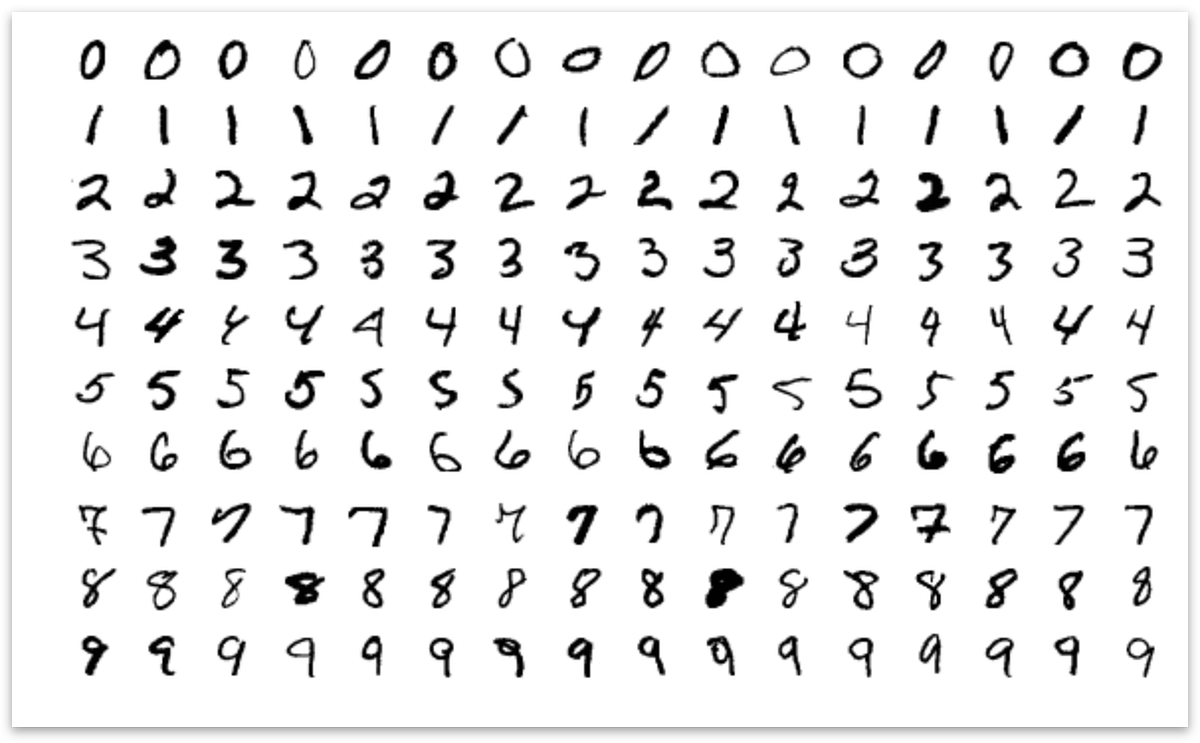
\includegraphics[width = \textwidth]{media/mnistDigit.png}
\end{center}

Während wir problemlos die Ziffern oben erkennen können, ist das für ein Computer keinesfalls einfach, weil die gleiche Ziffer ganz unterschiedlich dargestellt werden kann.
Für diese Fälle hat man in den vergangenen Jahren mit neuronalen Netzen grosse Erfolge erzielt. Dabei wird das Programm zuerst «trainiert», damit der Computer die richtigen Muster «erlernt». Im Grunde geht das wie folgt:

\begin{center}
	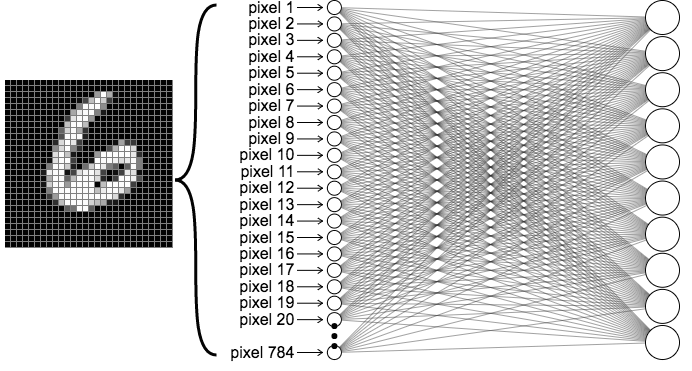
\includegraphics[width = \textwidth]{media/MnistArchitecture.png}
\end{center}


Das Programm erhält als Eingabe ein Bild. Im Beispiel handelt es sich um ein Schwarzweiss-Bild mit \( 28 \times 28 = 784 \) Pixeln.

Dieses Input-Bild kann als Vektor \( \vec{v} \) mit 784 Komponenten interpretiert werden. In der \( 30 \)-sten Komponente steht zum Beispiel, wie dunkel der entsprechende Pixel (2. Pixel in der 2. Zeile) ist – auf einer Skala von 0 bis 1.

\medskip

Dieser Vektor wird mit einer \( 10 \times 784 \)-Matrix \( M \) multipliziert\footnote{Das ist die Grundidee. In Wahrheit ist es etwas komplizierter.}. Damit erhält man einen neuen Vektor
\[
	\vec{w} = M \cdot \vec{v}
\]
mit 10 Einträgen. In diesem Vektor \( \vec{w} \) steht, wie wahrscheinlich das Bild eine bestimmte Ziffer darstellt:

\begin{itemize}
	\item Der 1. Eintrag steht für die Wahrscheinlichkeit, dass die Ziffer eine Eins ist,
	\item der 4. Eintrag z.\,B. für eine Vier,
	\item der 10. Eintrag für eine Null.
\end{itemize}

\medskip

\textbf{Zentrale Frage:} Wie lauten die 7840 Einträge der Matrix \( M \)?

Die Kernidee des \emph{maschinellen Lernens} ist, dass der Computer diese Einträge \textbf{selbstständig lernen} kann!

\medskip

Zunächst beginnt man mit einer zufälligen Startmatrix \( M \) und verbessert diese schrittweise. Dazu verwendet man ein bekanntes Eingabebild – zum Beispiel das einer 6 – und berechnet den Output-Vektor:
\[
	\vec{w} = M \cdot \vec{v}
\]


Die Komponenten des Vektors \( \vec{w} \) sind zu Beginn meist zufällig verteilt, etwa so:
\[
	\vec{w} =
	\begin{pmatrix}
		0.2 \\
		0.1 \\
		0.8 \\
		0.6 \\
		0.2 \\
		0.4 \\
		0.6 \\
		0.9 \\
		0.3 \\
		0.1
	\end{pmatrix}
\]

Da das Bild eine \textbf{Sechs} darstellt, sollte idealerweise jeder Eintrag des Outputvektors \( \vec{w} \) gleich null sein – mit Ausnahme des sechsten Eintrags, der den Wert 1 haben sollte.

\medskip

So entsteht ein \textbf{Fehlervektor}:
\[
	\vec{f} = \vec{w} - \vec{z} =
	\begin{pmatrix}
		-0.2 \\
		-0.1 \\
		-0.8 \\
		-0.6 \\
		-0.2 \\
		0.6  \\
		-0.6 \\
		-0.9 \\
		-0.3 \\
		-0.1
	\end{pmatrix}
\]
wobei \( \vec{z} \) der Zielvektor ist mit Eins an sechster Stelle und sonst Nullen.

\medskip

Das \textbf{Quadrat der Länge} des Fehlervektors ergibt den Fehlerwert:
\[
	F = |\vec{f}|^2 = (-0.2)^2 + (-0.1)^2 + \cdots + (-0.1)^2
\]

Offensichtlich hängt die Grösse von \( F \) von den Einträgen $m_{1,1}, m_{1,2}, \dotsc, m_{10,784}$ der Matrix \( M \) ab.
Man kann \( F \) daher als Funktion
\[
	F = F\left(m_{1,1}, m_{1,2}, \dotsc, m_{10,784}\right)
\]
auffassen – also eine Funktion in 7840 Variablen!

\medskip

Im Lernprozess wird die Matrix \( M \) nun so verändert, dass der Fehler \( F \) kleiner wird.
Hier kommt der \textbf{Gradient} ins Spiel:
Die grösste Abnahme von \( F \) geschieht in Richtung \( -\vec{\nabla}F \).

\medskip

Man erhält eine neue Matrix \( M_{\text{neu}} \), deren Einträge aus der Summe der entsprechenden Einträge von \( M \) und \( -\vec{\nabla}F \) gebildet werden:
\[
	M_{\text{neu}} = M - k \cdot \vec{\nabla}F
\]
(wobei \( k \) die sogenannte `Lernrate' ist).

\medskip

Dieser Vorgang wird wiederholt – jeweils mit unterschiedlichen Trainingsbildern –, bis das Programm die gewünschten Ergebnisse liefert.














\begin{LA}
	{Aufgabe: Anwendung des Gradienten auf neuronale Netzwerke}{}


	Ein Computerprogramm soll mit einem (vereinfachten) neuronalen Netzwerk lernen, Zahlen zu addieren und zu subtrahieren.

	Das Programm erhält als Input zwei Zahlen \( v_1 \) und \( v_2 \), die wir als Vektor
	\[
		\vec{v} = \begin{pmatrix} v_1 \\ v_2 \end{pmatrix}
	\]
	auffassen, und berechnet den Output
	\[
		\vec{w} = \begin{pmatrix} w_1 \\ w_2 \end{pmatrix} = M \cdot \vec{v},
	\]
	wobei \( M \) eine \( 2 \times 2 \)-Matrix ist, die zu Beginn zufällig gewählt ist und mit dem Gradient-Descent-Verfahren laufend verbessert werden soll, sodass der gewünschte Zieloutput
	\[
		\vec{z} = \begin{pmatrix} v_1 + v_2 \\ v_1 - v_2 \end{pmatrix}
	\]
	damit berechnet wird.

	\medskip

	Zu Beginn soll die Matrix die Einträge
	\[
		M = \begin{pmatrix} 1 & 2 \\ 3 & 4 \end{pmatrix}
	\]
	aufweisen. Das neuronale Netzwerk wird mit der Eingabe
	\[
		\vec{v} = \begin{pmatrix} 2 \\ 1 \end{pmatrix}
	\]
	trainiert.

	\begin{itemize}
		\item Berechnen Sie den Output \( \vec{w} \) des neuronalen Netzwerks, den Fehlervektor \( \vec{f} = \vec{w} - \vec{z} \) und dessen quadrierten Betrag \( F = |\vec{f}|^2 \).\\
		      \textit{(Kontrolle: \( \vec{w} = \begin{pmatrix} 4 \\ 10 \end{pmatrix} \), \( \vec{f} = \begin{pmatrix} 1 \\ 9 \end{pmatrix} \), \( F = 82 \))}
	\end{itemize}

	Als nächstes soll die Matrix so verändert werden, dass der Fehler kleiner wird. Dazu betrachten wir den Fehler \( F \) als Funktion der Einträge der Matrix
	\[
		M = \begin{pmatrix} a & b \\ c & d \end{pmatrix}.
	\]

	\begin{itemize}
		\item Berechnen Sie nochmals den Fehler \( F = |\vec{f}|^2 \) mit dem Input \( \vec{v} = \begin{pmatrix} 2 \\ 1 \end{pmatrix} \), wobei \( M \) nun allgemein \( \begin{pmatrix} a & b \\ c & d \end{pmatrix} \) ist.\\
		      \textit{(Kontrolle: \( F(a,b,c,d) = (2a + b - 3)^2 + (2c + d - 1)^2 \))}
	\end{itemize}

	Den Fehler fassen wir ab jetzt als Funktion mit vier Argumenten \( a, b, c, d \) auf.
	Den Graphen von \( F \) könnte man als 4-dimensionale Hyperfläche in einem 5-dimensionalen Raum realisieren.
	Hier versagt die Vorstellungskraft – wir können aber die Ideen der Funktionen in zwei Variablen nutzen!

	\medskip

	Wir ändern die Inputs \( a, b, c, d \) (also die Einträge der Matrix \( M \)) so, dass der Fehler kleiner wird.
	Wie stark soll jeder Eintrag verändert werden? Der Gradient liefert die Antwort:

	\begin{itemize}
		\item Berechnen Sie den Gradienten \( \vec{\nabla}F \) der Funktion \( F(a,b,c,d) \) an der Stelle \( (a_0, b_0, c_0, d_0) = (1, 2, 3, 4) \).\\
		      \textit{(Kontrolle: \( \vec{\nabla}F(1,2,3,4) = \begin{pmatrix} 4 \\ 2 \\ 36 \\ 18 \end{pmatrix} \))}
	\end{itemize}

	Der Gradient zeigt in Richtung des stärksten Anstiegs der Fehlerfunktion \( F \).
	Um die Einträge der Matrix \( M \) so zu verändern, dass der Fehler kleiner wird, müssen diese also in Richtung \( -\vec{\nabla}F \) verändert werden.

	\medskip

	Allerdings sind die Einträge des Gradienten sehr gross.
	Wenn wir die Einträge der Matrix \( M \) einen Schritt in Richtung Gradient verändern, würden wir an den Werten für den minimalen Fehler «vorbeischiessen».
	Aus diesem Grund verändern wir die Einträge nur um \( \frac{1}{20} \cdot \vec{\nabla}F \).
	(Der Faktor \( k = \frac{1}{20} \) heisst \emph{Lernrate}.)

	\begin{itemize}
		\item Fassen Sie die Matrix \( M = \begin{pmatrix} 1 & 2 \\ 3 & 4 \end{pmatrix} \) als Vektor \( \vec{m} = \begin{pmatrix} 1 \\ 2 \\ 3 \\ 4 \end{pmatrix} \) auf. Berechnen Sie:
		      \[
			      \vec{m}_{\text{neu}} = \vec{m} - \frac{1}{20} \cdot \vec{\nabla}F(1,2,3,4)
		      \]
		      Wandeln Sie das Resultat wieder in eine Matrix \( M_{\text{neu}} \) um und berechnen Sie den neuen Fehler \( F_{\text{neu}} \).\\
		      \textit{(Kontrolle: \( F_{\text{neu}} = 20.5 \))}
	\end{itemize}

	Der Wert der Fehlerfunktion \( F \) ist deutlich kleiner geworden.
	Wird dieses Training mehrmals mit unterschiedlichen Eingaben durchgeführt, so nähert sich die Matrix \( M \) schrittweise der Matrix
	\[
		M_\infty = \begin{pmatrix} 1 & 1 \\ 1 & -1 \end{pmatrix}.
	\]

	Auf diese Art lernt das Programm, welche Werte die Matrix haben muss, um zwei Zahlen zu addieren und zu subtrahieren.

	\bigskip

	\textbf{Zusatzfrage:}
	Zeigen Sie: Hätten wir als Lernrate \( \frac{1}{10} \) gewählt, hätten wir \( F_{\text{neu}} = 0 \) erhalten.
	Die Matrix \( M_{\text{neu}} \) berechnet aber nur \emph{für diesen Vektor} den richtigen Output.
	In Wirklichkeit wird das neuronale Netzwerk mit ganz vielen unterschiedlichen In- und Ziel-Outputs trainiert.

\end{LA}

























\clearpage
\subsection{Vermischte Aufgaben}
\begin{ueb}
	{}{}
	\begin{enumerate}
		\item Bestimmen Sie den Gradienten der folgenden Funktionen:
		      \begin{enumerate}
			      \item \( f(x, y) = x^2 + y^2 \)
			      \item \( g(x, y) = e^{x - y} \)
			      \item \( h(x, y) = \sin(x) \cdot \cos(y) \)
		      \end{enumerate}

		\item
		      Betrachten wir einen Massenpunkt, der im Ursprung unseres Koordinatensystems so gelagert ist, dass seine Auslenkung in Richtung der Koordinatenachsen, etwa durch zwei Federn realisiert, eine Rückstellkraft proportional zur Auslenkung erfährt, die in $y$-Richtung doppelt so gross sei, wie in $x$-Richtung.
		      \begin{center}
			      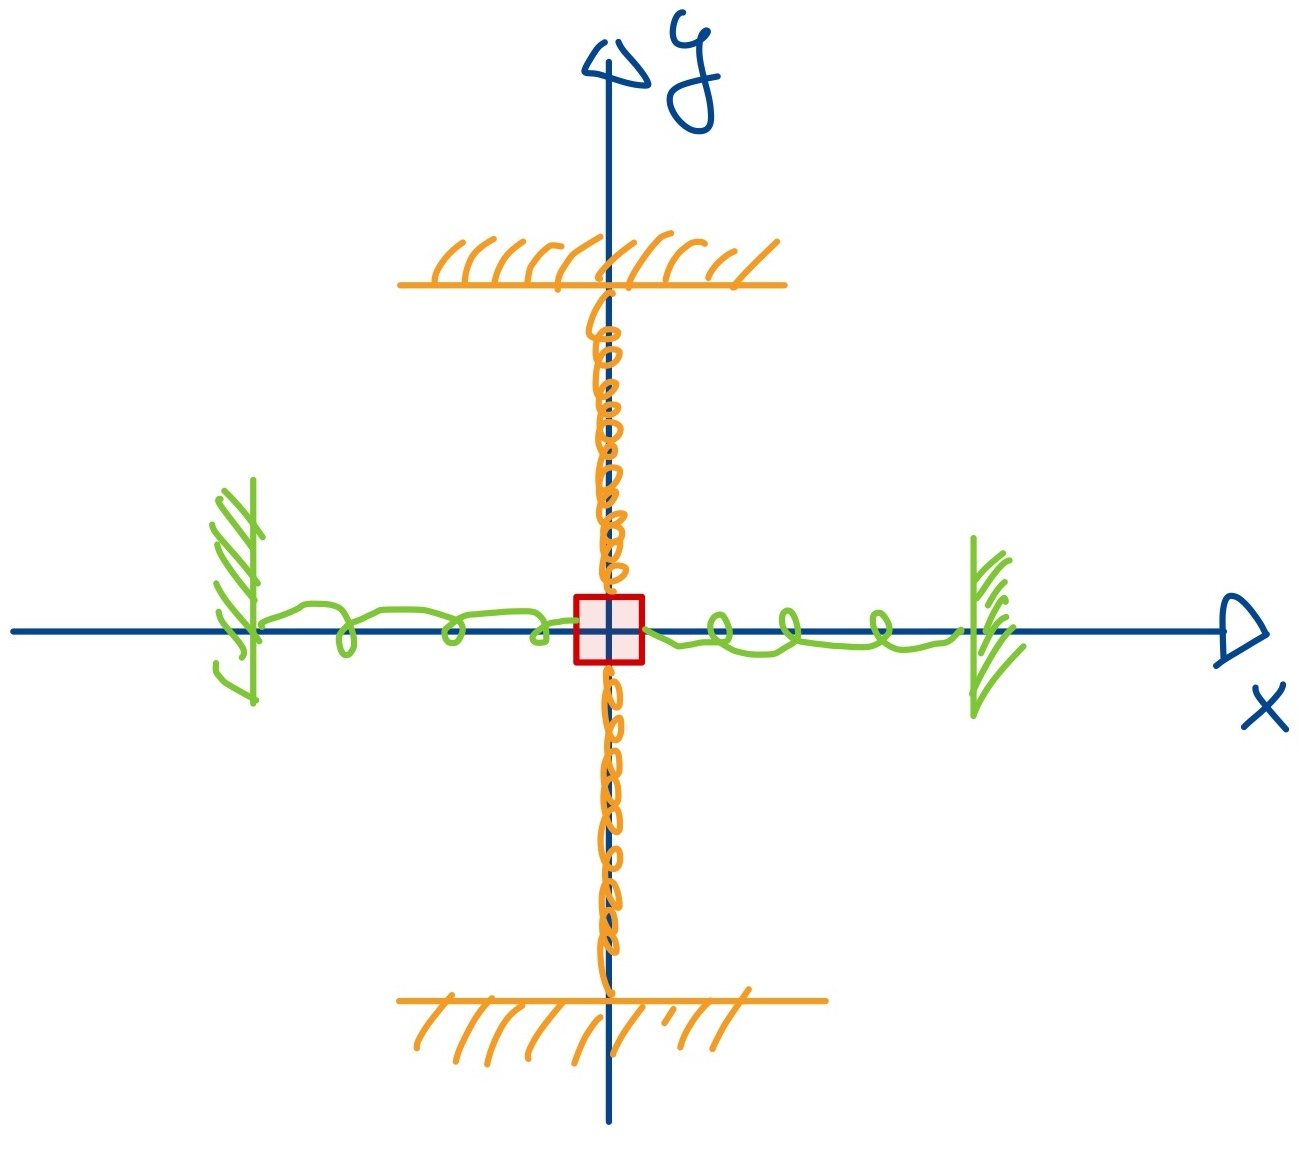
\includegraphics[width = 0.4\textwidth]{media/harm-osz-1.jpg}
		      \end{center}

		      Die potenzielle Energie $V(x,y)$ bei einer Auslenkung $(x,y)$ aus der Ruhelage ist dann (Bei Federkonstanten 1 bzw. 2):
		      \[
			      V(x, y) = \frac{1}{2}x^2 + y^2
		      \]
		      \begin{enumerate}
			      \item Geben Sie die Gleichung der Niveaulinie \( N_1 \) zum Wert \( V = 1 \) an. Es handelt sich um eine Ellipse!
			            Geben Sie die Halbachsen an und fertigen Sie eine Skizze.

			            \emph{Hinweis}: Ellipsen haben eine Gleichung der Form
			            $$\frac{x^2}{a^2} + \frac{y^2}{b^2} = 1$$
			            mit den Halbachsen \( a \) und \( b \).
			      \item Zeigen Sie, dass der Punkt \( P = \left( 1, \frac{\sqrt{2}}{2} \right) \) auf \( N_1 \) liegt.
			      \item Berechnen Sie den Gradienten an der Stelle \( P \). Welche Bedeutung hat das Resultat im Kontext des harmonischen Oszillators?
			      \item Geben Sie die Gleichung der Tangente an \( N_1 \) im Punkt \( P \) an.
		      \end{enumerate}

		\item Die Temperatur einer in der \( xy \)-Ebene liegenden Platte sei gegeben durch:
		      \[
			      T(x, y) = \frac{1}{1 + x^2 + y^2}, \qquad x,y \text{ Position in Meter, } \quad T \text{ in Grad Celsius}
		      \]
		      \begin{enumerate}
			      \item Berechnen Sie den Gradienten in jedem Punkt.
			      \item In welche Richtung ist der Temperaturanstieg am grössten?
			      \item Schliessen Sie vom Gradienten auf die Gestalt der Niveaulinien.
			      \item Ein Massenpunkt bewegt sich entlang einer Geraden in Richtung $\begin{pmatrix}
					            1 \\ 3
				            \end{pmatrix}$. Berechnen Sie den lokalen Temperaturanstieg in Grad Celsius/Meter beim Passieren des Punktes \( (2, 3) \) in Richtung der Geraden.
			            % \(
			            % \begin{pmatrix}
			            % 1 \\ 3
			            % \end{pmatrix}
			            % \)
			            %in \( ^\circ\mathrm{C}/\mathrm{LE} \).
		      \end{enumerate}

		\item Durch ein Gelände mit der Höhenfunktion
		      \[
			      h(x, y) = \frac{1000 + x + y + \sqrt{xy + 76}}{10}
		      \]
		      wird längs der Geraden
		      \[
			      \vec{r}(t) = \begin{pmatrix} 1 \\ 2 \end{pmatrix} + t \cdot \begin{pmatrix} 3 \\ 4 \end{pmatrix}
		      \]
		      eine Strasse gebaut. Bestimmen Sie die Steigung der Strasse an der Stelle \( (x, y) = (4, 6) \).

		\item Gegeben sei die Funktion
		      \[
			      f(x, y) = \sin(x) + \sin(y) + \sin(x + y)
		      \]
		      \begin{enumerate}
			      \item Wie gross ist die Steigung der Tangente an die Schnittkurve des Graphen von \( f \) mit einer zur \( xz \)-Ebene parallelen Ebene im Punkt \( P = \left( \frac{\pi}{2}, \frac{\pi}{4}, ? \right) \)?
			      \item Geben Sie eine Gleichung der Tangentialebene an den Graphen im Ursprung an.
		      \end{enumerate}
	\end{enumerate}
\end{ueb}



\clearpage
\emph{Lösungen}


\begin{enumerate}
	\item \textbf{Gradienten}
	      \begin{enumerate}
		      \item \( \vec{\nabla} f(x, y) = 2 \begin{pmatrix} x \\ y \end{pmatrix} \)
		      \item \( \vec{\nabla} g(x, y) = e^{x - y} \begin{pmatrix} 1 \\ -1 \end{pmatrix} \)
		      \item \( \vec{\nabla} h(x, y) = \begin{pmatrix}
			            \cos(x) \cos(y) \\
			            -\sin(x) \sin(y)
		            \end{pmatrix} \)
	      \end{enumerate}

	\item \textbf{Harmonischer Oszillator}
	      \begin{enumerate}
		      \item Niveaulinie \( N_1 \): \( \frac{x^2}{2} + y^2 = 1 \)
		            Ellipse mit Halbachsen \( \sqrt{2} \) und \( 1 \).
		      \item \( V\left(1, \frac{\sqrt{2}}{2}\right) = \frac{1}{2} + \frac{1}{2} = 1 \)
		      \item \( \vec{\nabla} V\left(1, \frac{\sqrt{2}}{2}\right) = \begin{pmatrix} 1 \\ \sqrt{2} \end{pmatrix} \) Bewegt sich der Massepunkt ausgehend von \( P \) in Richtung des Gradienten, so steigt die Energie am schnellsten an.
		      \item Tangente an \( N_1 \) im Punkt \( P \):
		            \[
			            \vec{r}(t) = \begin{pmatrix} 1 \\ \frac{\sqrt{2}}{2} \end{pmatrix} + t \cdot \begin{pmatrix} -\sqrt{2} \\ 1 \end{pmatrix}
			            \quad \text{oder} \quad y = -\frac{\sqrt{2}}{2} x + \sqrt{2}
		            \]
	      \end{enumerate}

	\item \textbf{Temperaturfeld}
	      \begin{enumerate}
		      \item Gradient:
		            \[
			            \vec{\nabla} T(x, y) = -\frac{2}{(1 + x^2 + y^2)^2} \begin{pmatrix} x \\ y \end{pmatrix}
		            \]
		      \item Der Temperaturanstieg ist in Richtung des Ursprungs am grössten.
		      \item Die Normale zur Niveaulinie zeigt stets zum Ursprung. Die Niveaulinien sind also Kreise mit Zentrum im Ursprung.
		      \item Richtungsableitung bei \( (2, 3) \) in die normierte Richtung \( \frac{1}{\sqrt{10}} \begin{pmatrix} 1 \\ 3 \end{pmatrix} \):
		            \[
			            \frac{\partial T}{\partial \vec{v}}(2, 3) = -\frac{11}{98\sqrt{10}}
		            \]
	      \end{enumerate}

	\item \textbf{Gelände und Strasse}
	      \begin{enumerate}
		      \item Steigung entlang \( \vec{v} = \begin{pmatrix} 3 \\ 4 \end{pmatrix} \) bei \( (4, 6) \):
		            \[
			            \frac{1}{5} \frac{\partial h}{\partial \vec{v}}(4, 6) = \frac{87}{500}
		            \]
	      \end{enumerate}

	\item \textbf{Funktion mit Sinus-Termen}
	      \begin{enumerate}
		      \item \(\frac{\partial f}{\partial x} \left(\frac{\pi}{2}, \frac{\pi}{4}\right) = -\frac{\sqrt{2}}{2} \)
		      \item Tangentialebene im Ursprung:
		            \[
			            T: z = 2x + 2y
		            \]
	      \end{enumerate}
\end{enumerate}
